% -*- TeX -*- -*- UK -*-
% ----------------------------------------------------------------
% arXiv Paper ************************************************
%
% Subhaneil Lahiri's template
%
% Before submitting:
%    Comment out hyperref
%    Comment out showkeys
%    Replace \newcommand{\mlim}[2]{{\stackrel{\scriptstyle #1}{#2}}}
\newcommand{\ra}{\rightarrow}
\newcommand{\lr}{\leftrightarrow}
\newcommand{\cdt}{\!\cdot\!}
\newcommand{\vp}{\vspace{0.5cm}}
\newcommand{\degs}{^\circ}
%
%e.g., i.e. with normal spaces
\newcommand{\eg}{e.g.\ }
\newcommand{\ie}{i.e.\ }
\newcommand{\cf}{cf.\ }
\newcommand{\etc}{etc.\ }
%
% indices
\newcommand{\up}[1]{\mbox{}^{#1}}
\newcommand{\dn}[1]{\mbox{}_{#1}}
\newcommand{\rp}[1]{^{(#1)}}
\newcommand{\lp}[1]{_{(#1)}}
%
% brackets etc.
\newcommand{\prn}[1]{\left ( #1 \right )}
\newcommand{\brc}[1]{\left\{ #1 \right\}}
\newcommand{\brk}[1]{\left [ #1 \right ]}
\newcommand{\abs}[1]{\left\lvert #1 \right\rvert}
\newcommand{\nrm}[1]{\left\lVert #1 \right\rVert}
\newcommand{\av}[1]{\left\langle #1 \right\rangle}
%
% QM Dirac notation
\newcommand{\bra}[1]{\left\langle #1 \right \rvert}
\newcommand{\ket}[1]{\left \lvert #1 \right\rangle}
\newcommand{\braket}[2]{\left\langle #1 \midddle | #2 \right\rangle}
\newcommand{\bracket}[3]{\left\langle #1 \middle | #2 \middle | #3 \right\rangle}
%
% Derivatives, etc. First argument is optional.
\newcommand{\diff}[3][\rule{0mm}{0mm}]{\frac{\mathrm{d}^{#1} #2}{\mathrm{d}{#3}^{#1}}}
\newcommand{\pdiff}[3][\rule{0mm}{0mm}]{\frac{\partial^{#1} #2}{\partial {#3}^{#1}}}
\newcommand{\pdiffc}[3][\rule{0mm}{0mm}]{\left (\frac{\partial #2}{\partial {#3}}\right )_{\!\!#1}}
\newcommand{\pdl}[1][\rule{0mm}{0mm}]{\overleftarrow{\partial}_{#1}}
\newcommand{\pdr}[1][\rule{0mm}{0mm}]{\overrightarrow{\partial}_{#1}}
\newcommand{\pdlr}[1][\rule{0mm}{0mm}]{\overleftrightarrow{\partial_{#1}}}
\newcommand{\fdf}[2]{\frac{\delta #1}{\delta #2}}
\newcommand{\intd}[1]{\int\!\dr #1\,}
%
% Un-italicised letters
\newcommand{\dr}{\mathrm{d}}
\newcommand{\e}{\mathrm{e}}
\newcommand{\ir}{\mathrm{i}}
\DeclareMathOperator{\tr}{tr}
\DeclareMathOperator{\Tr}{Tr}
\DeclareMathOperator{\Det}{Det}
%
% The default \Im and \Re look crap
\renewcommand{\Im}{\operatorname{\mathfrak{Im}}}
\renewcommand{\Re}{\operatorname{\mathfrak{Re}}}
%
% Referencing sections, figures, etc
\newcommand{\sref}[1]{\S\ref{#1}}
\newcommand{\cref}[1]{Ch.\ref{#1}}
\newcommand{\Cref}[1]{Ch.\ref{#1}}
\newcommand{\fref}[1]{fig.\ref{#1}}
\newcommand{\Fref}[1]{Fig.\ref{#1}}
\newcommand{\tref}[1]{tab.\ref{#1}}
\newcommand{\Tref}[1]{Tab.\ref{#1}}
%
\newcommand{\nn}{\nonumber}
%
% Put the preprint numbers in the top right corner of the page.
% Use after \maketitle.
% First argument: How high it needs to be raised,
% Second argument: Width of the box,
% Third argument: The preprint numbers.
\newcommand{\preprintno}[3]{\hfill\raisebox{#1}[0cm][0cm]{
\begin{minipage}[t]{#2}\begin{flushright} #3 \end{flushright}\end{minipage}}
\vspace*{-\baselinestretch\baselineskip}}
%
% If you have changed the line spacing, e.g. with \renewcommand{\baselinestretch}{1.5},
% the command \sgap produces a line break with the normal spacing.
\newlength{\lingap}
\setlength{\lingap}{\baselinestretch\baselineskip}
\addtolength{\lingap}{-\baselineskip}
\newcommand{\sgap}{\\[-\lingap]}
 with its contents
%       or include mydefs.tex in zip/tar file
%    Replace %
\newcommand{\CD}{\mathcal{D}}
\newcommand{\CE}{\mathcal{E}}
\newcommand{\CG}{\mathcal{G}}
\newcommand{\CH}{\mathcal{H}}
\newcommand{\CK}{\mathcal{K}}
\newcommand{\CO}{\mathcal{O}}
\newcommand{\CL}{\mathcal{L}}
\newcommand{\CM}{\mathcal{M}}
\newcommand{\CN}{\mathcal{N}}
\newcommand{\CV}{\mathcal{V}}
\newcommand{\CZ}{\mathcal{Z}}
%
\newcommand{\dM}{\mathfrak{M}}
\newcommand{\dmd}{\mathfrak{d}}
\newcommand{\dmD}{\mathfrak{D}}
%
\newcommand{\R}{\mathbb{R}}
\newcommand{\C}{\mathbb{C}}
\newcommand{\CP}{\mathbb{CP}}
\newcommand{\Z}{\mathbb{Z}}
%
\newcommand{\ad}{{\dot{\alpha}}}
\newcommand{\bd}{{\dot{\beta}}}
\newcommand{\gd}{{\dot{\gamma}}}
\newcommand{\dd}{{\dot{\delta}}}
\newcommand{\ed}{{\dot{\epsilon}}}
%
\newcommand{\bs}{\overline{\sigma}}
\newcommand{\br}{\overline{\rho}}
\newcommand{\bpsi}{\overline{\psi}}
\newcommand{\bchi}{\overline{\chi}}
\newcommand{\bPsi}{\overline{\Psi}}
\newcommand{\bQ}{\overline{Q}}
\newcommand{\bS}{\overline{S}}
\newcommand{\bJ}{\overline{J}}
\newcommand{\zb}{{\bar z}}
\newcommand{\wb}{{\overline w}}
\newcommand{\cb}{{\bar c}}
\newcommand{\ab}{{\bar a}}
\newcommand{\bb}{{\bar b}}
\newcommand{\bp}{{\bar\partial}}
%
\newcommand{\p}{\partial}
\newcommand{\apm}{{\alpha^{\prime}}}
\newcommand{\adg}{a^\dagger}
\newcommand{\psq}{^{\prime\,2}}
\newcommand{\ppsq}{^{\prime\prime\,2}}
\newcommand{\half}{\frac{1}{2}}
%
 with its contents
%       or include newsymb.tex in zip/tar file
%    Put this file, the .bbl file, any picture or
%       other additional files and natbib.sty
%       file in a zip/tar file
%
% **** -----------------------------------------------------------
\documentclass[12pt]{article}
% Preamble:
\usepackage{a4wide}
\usepackage{multirow}
\usepackage[centertags]{amsmath}
\usepackage{amssymb}
%\usepackage{amsthm}
\usepackage[sort&compress,numbers]{natbib}
%\usepackage{citeB}
\usepackage{ifpdf}
\usepackage{graphicx}
%\usepackage{graphics} for finding documentation only
%\usepackage{xcolor}
%\usepackage{pgf}
\ifpdf
\usepackage[pdftex,bookmarks]{hyperref}
\else
\usepackage[hypertex]{hyperref}
\DeclareGraphicsRule{.png}{eps}{.bb}{}
\fi
\usepackage{epstopdf}
\epstopdfsetup{update,suffix=-generated}
%
% >> Only for drafts! <<
\usepackage[notref,notcite]{showkeys}
% ----------------------------------------------------------------
\vfuzz2pt % Don't report over-full v-boxes if over-edge is small
\hfuzz2pt % Don't report over-full h-boxes if over-edge is small
%\numberwithin{equation}{section}
%\renewcommand{\baselinestretch}{1.5}
% ----------------------------------------------------------------
% New commands etc.
\newcommand{\mlim}[2]{{\stackrel{\scriptstyle #1}{#2}}}
\newcommand{\ra}{\rightarrow}
\newcommand{\lr}{\leftrightarrow}
\newcommand{\cdt}{\!\cdot\!}
\newcommand{\vp}{\vspace{0.5cm}}
\newcommand{\degs}{^\circ}
%
%e.g., i.e. with normal spaces
\newcommand{\eg}{e.g.\ }
\newcommand{\ie}{i.e.\ }
\newcommand{\cf}{cf.\ }
\newcommand{\etc}{etc.\ }
%
% indices
\newcommand{\up}[1]{\mbox{}^{#1}}
\newcommand{\dn}[1]{\mbox{}_{#1}}
\newcommand{\rp}[1]{^{(#1)}}
\newcommand{\lp}[1]{_{(#1)}}
%
% brackets etc.
\newcommand{\prn}[1]{\left ( #1 \right )}
\newcommand{\brc}[1]{\left\{ #1 \right\}}
\newcommand{\brk}[1]{\left [ #1 \right ]}
\newcommand{\abs}[1]{\left\lvert #1 \right\rvert}
\newcommand{\nrm}[1]{\left\lVert #1 \right\rVert}
\newcommand{\av}[1]{\left\langle #1 \right\rangle}
%
% QM Dirac notation
\newcommand{\bra}[1]{\left\langle #1 \right \rvert}
\newcommand{\ket}[1]{\left \lvert #1 \right\rangle}
\newcommand{\braket}[2]{\left\langle #1 \midddle | #2 \right\rangle}
\newcommand{\bracket}[3]{\left\langle #1 \middle | #2 \middle | #3 \right\rangle}
%
% Derivatives, etc. First argument is optional.
\newcommand{\diff}[3][\rule{0mm}{0mm}]{\frac{\mathrm{d}^{#1} #2}{\mathrm{d}{#3}^{#1}}}
\newcommand{\pdiff}[3][\rule{0mm}{0mm}]{\frac{\partial^{#1} #2}{\partial {#3}^{#1}}}
\newcommand{\pdiffc}[3][\rule{0mm}{0mm}]{\left (\frac{\partial #2}{\partial {#3}}\right )_{\!\!#1}}
\newcommand{\pdl}[1][\rule{0mm}{0mm}]{\overleftarrow{\partial}_{#1}}
\newcommand{\pdr}[1][\rule{0mm}{0mm}]{\overrightarrow{\partial}_{#1}}
\newcommand{\pdlr}[1][\rule{0mm}{0mm}]{\overleftrightarrow{\partial_{#1}}}
\newcommand{\fdf}[2]{\frac{\delta #1}{\delta #2}}
\newcommand{\intd}[1]{\int\!\dr #1\,}
%
% Un-italicised letters
\newcommand{\dr}{\mathrm{d}}
\newcommand{\e}{\mathrm{e}}
\newcommand{\ir}{\mathrm{i}}
\DeclareMathOperator{\tr}{tr}
\DeclareMathOperator{\Tr}{Tr}
\DeclareMathOperator{\Det}{Det}
%
% The default \Im and \Re look crap
\renewcommand{\Im}{\operatorname{\mathfrak{Im}}}
\renewcommand{\Re}{\operatorname{\mathfrak{Re}}}
%
% Referencing sections, figures, etc
\newcommand{\sref}[1]{\S\ref{#1}}
\newcommand{\cref}[1]{Ch.\ref{#1}}
\newcommand{\Cref}[1]{Ch.\ref{#1}}
\newcommand{\fref}[1]{fig.\ref{#1}}
\newcommand{\Fref}[1]{Fig.\ref{#1}}
\newcommand{\tref}[1]{tab.\ref{#1}}
\newcommand{\Tref}[1]{Tab.\ref{#1}}
%
\newcommand{\nn}{\nonumber}
%
% Put the preprint numbers in the top right corner of the page.
% Use after \maketitle.
% First argument: How high it needs to be raised,
% Second argument: Width of the box,
% Third argument: The preprint numbers.
\newcommand{\preprintno}[3]{\hfill\raisebox{#1}[0cm][0cm]{
\begin{minipage}[t]{#2}\begin{flushright} #3 \end{flushright}\end{minipage}}
\vspace*{-\baselinestretch\baselineskip}}
%
% If you have changed the line spacing, e.g. with \renewcommand{\baselinestretch}{1.5},
% the command \sgap produces a line break with the normal spacing.
\newlength{\lingap}
\setlength{\lingap}{\baselinestretch\baselineskip}
\addtolength{\lingap}{-\baselineskip}
\newcommand{\sgap}{\\[-\lingap]}

%
\newcommand{\CD}{\mathcal{D}}
\newcommand{\CE}{\mathcal{E}}
\newcommand{\CG}{\mathcal{G}}
\newcommand{\CH}{\mathcal{H}}
\newcommand{\CK}{\mathcal{K}}
\newcommand{\CO}{\mathcal{O}}
\newcommand{\CL}{\mathcal{L}}
\newcommand{\CM}{\mathcal{M}}
\newcommand{\CN}{\mathcal{N}}
\newcommand{\CV}{\mathcal{V}}
\newcommand{\CZ}{\mathcal{Z}}
%
\newcommand{\dM}{\mathfrak{M}}
\newcommand{\dmd}{\mathfrak{d}}
\newcommand{\dmD}{\mathfrak{D}}
%
\newcommand{\R}{\mathbb{R}}
\newcommand{\C}{\mathbb{C}}
\newcommand{\CP}{\mathbb{CP}}
\newcommand{\Z}{\mathbb{Z}}
%
\newcommand{\ad}{{\dot{\alpha}}}
\newcommand{\bd}{{\dot{\beta}}}
\newcommand{\gd}{{\dot{\gamma}}}
\newcommand{\dd}{{\dot{\delta}}}
\newcommand{\ed}{{\dot{\epsilon}}}
%
\newcommand{\bs}{\overline{\sigma}}
\newcommand{\br}{\overline{\rho}}
\newcommand{\bpsi}{\overline{\psi}}
\newcommand{\bchi}{\overline{\chi}}
\newcommand{\bPsi}{\overline{\Psi}}
\newcommand{\bQ}{\overline{Q}}
\newcommand{\bS}{\overline{S}}
\newcommand{\bJ}{\overline{J}}
\newcommand{\zb}{{\bar z}}
\newcommand{\wb}{{\overline w}}
\newcommand{\cb}{{\bar c}}
\newcommand{\ab}{{\bar a}}
\newcommand{\bb}{{\bar b}}
\newcommand{\bp}{{\bar\partial}}
%
\newcommand{\p}{\partial}
\newcommand{\apm}{{\alpha^{\prime}}}
\newcommand{\adg}{a^\dagger}
\newcommand{\psq}{^{\prime\,2}}
\newcommand{\ppsq}{^{\prime\prime\,2}}
\newcommand{\half}{\frac{1}{2}}
%

\newcommand{\Pa}{\,\mathrm{Pa}}
\newcommand{\kg}{\,\mathrm{kg}}
\newcommand{\m}{\,\mathrm{m}}
\newcommand{\s}{\,\mathrm{s}}
\newcommand{\mins}{\,\mathrm{min}}
\newcommand{\N}{\,\mathrm{N}}
\newcommand{\g}{\,\mathrm{g}}
\newcommand{\cm}{\,\mathrm{cm}}
\newcommand{\Hz}{\,\mathrm{Hz}}
\newcommand{\J}{\,\mathrm{J}}
\newcommand{\K}{\,\mathrm{K}}
\newcommand{\eV}{\,\mathrm{eV}}
\newcommand{\MeV}{\,\mathrm{MeV}}
\newcommand{\GeV}{\,\mathrm{GeV}}
\newcommand{\TeV}{\,\mathrm{TeV}}
%\newcommand{\C}{\,\mathrm{C}}
\newcommand{\A}{\,\mathrm{A}}
\newcommand{\V}{\,\mathrm{V}}
\newcommand{\T}{\,\mathrm{T}}
\newcommand{\F}{\,\mathrm{F}}
\newcommand{\dC}{^\circ\mathrm{C}}
\newcommand{\degs}{^\circ}

%
%%%%%%%%%%%%%%%%%%%%%%%%%%%%%%%%%%%%%%%%%%%%%%%%%%%%%%%%%%%%%%%%%%%%%%%%%%
% Title info:
\title{Mutual information between successive reorientations}
%
% Author List:
%
\author{Subhaneil Lahiri
\\
%
% Addresses:
%
\small{\emph{Harvard University}}
%
}

\begin{document}

\maketitle



%%%%%%%%%%%%%%%%%%%%%%%%%%%%%%%%%%%%%%%%%%%%%%%%%%%%%%%%%%%%%%%%%%%%%%%%%%


\begin{abstract}
  We show how mutual information can be used to describe the independence of successive reorientations
\end{abstract}

\tableofcontents
\listoffigures
\listoftables

%%%%%%%%%%%%%%%%%%%%%%%%%%%%%%%%%%%%%%%%%%%%%%%%%%%%%%%%%%%%%%%%%%%%%%%%%%
% Beginning of Article:
%%%%%%%%%%%%%%%%%%%%%%%%%%%%%%%%%%%%%%%%%%%%%%%%%%%%%%%%%%%%%%%%%%%%%%%%%%

\section{Reorientation sequences}\label{sec:reoseq}

As a worm navigates, it performs a sequence of turns. When turns occur sufficiently close to each other, they are grouped into a reorientation event. Some example tracks, consisting of runs and reorientations, are shown in \fref{fig:tracks}. These reorientations have several characteristics, \eg the types of turn of which it is composed, the difference in heading direction before and after, the duration of the run leading into it. We wish to know if the characteristics of one reorientation are independent of the characteristics of previous reorientations.

Consider a sequence of $r$ successive reorientations. The values of a particular characteristic of these reorientations is an $r$-tuple of random variables\footnote{ Actually, reorientation type is not a random variable, as it is not described by a number. However, the concept of a probability distribution still makes sense, and the probability of the outcome can be considered a random variable. }: $(X_1,\ldots,X_r)$. We are asking whether or not $P(X_1,\ldots,X_r) = P(X_1)\ldots P(X_r)$. We will discuss some measures of independence in \sref{sec:entropy}.

These probability distributions can be estimated from the frequencies in a sample sequence (described schematically in \fref{fig:schematic}). However, as a consequence of finite sample size, this process has both systematic and random errors. We will look at several methods for removing systematic errors in \sref{sec:syscorr} and one method for estimating random errors in appendix \ref{sec:stderr}.

%\begin{figure}
%  (a)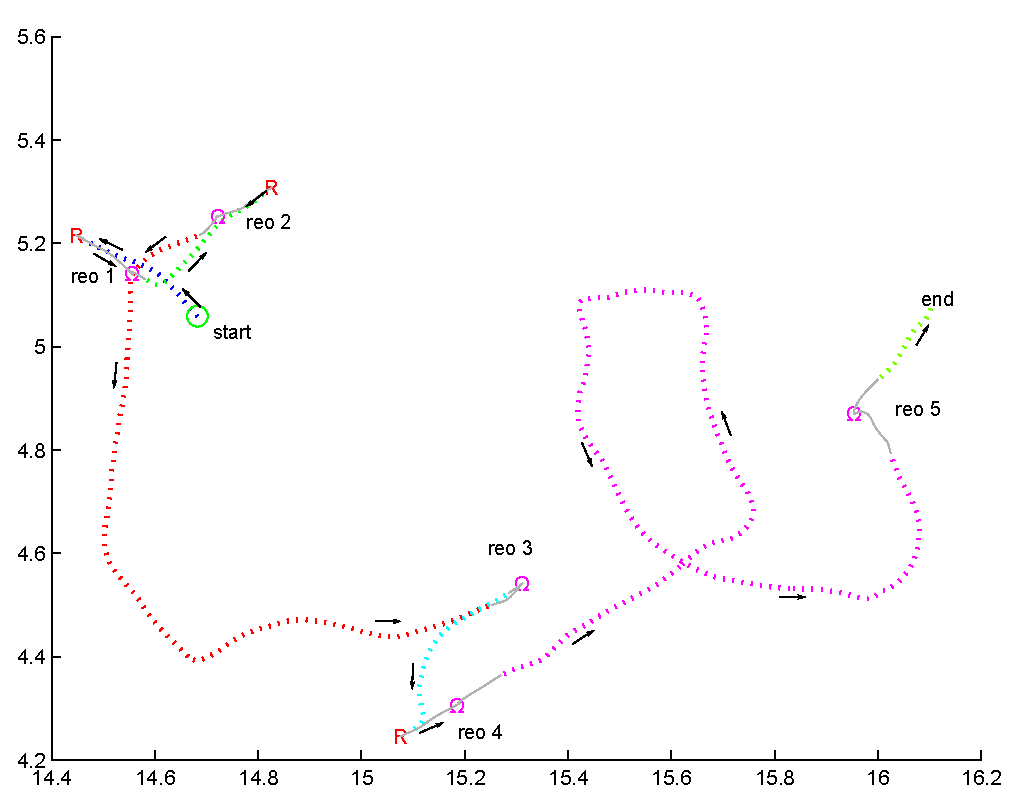
\includegraphics[width=6cm]{track1.eps}
%  (b)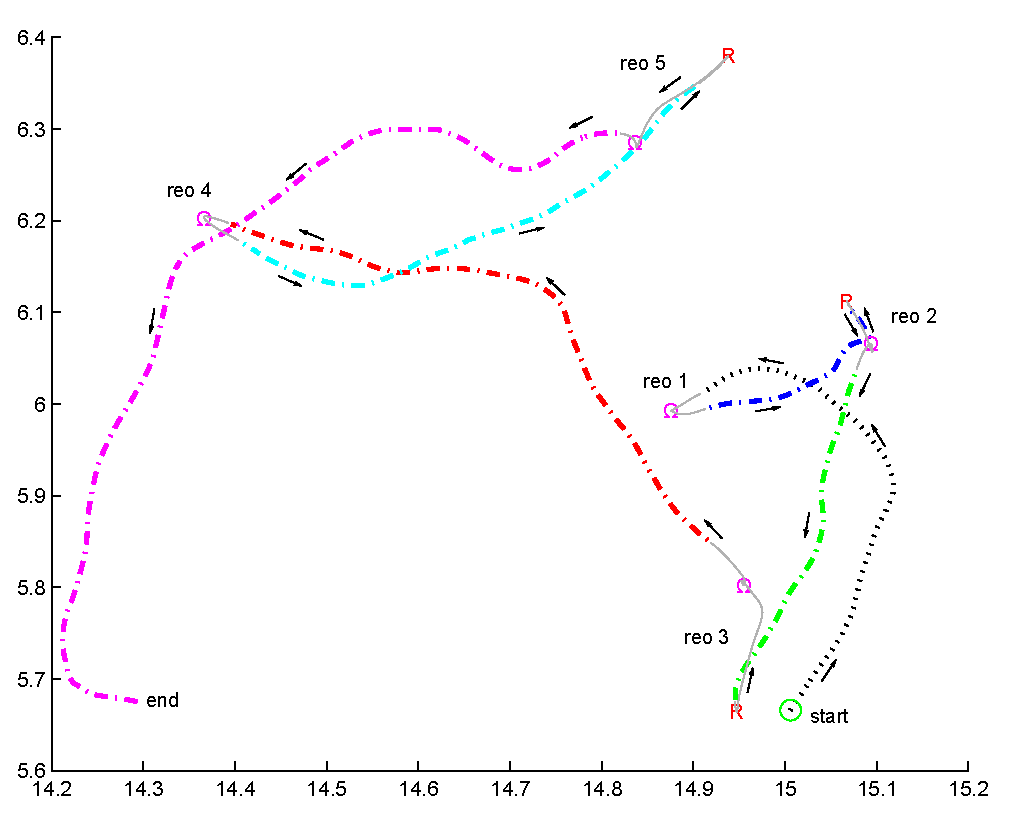
\includegraphics[width=6cm]{track2.eps}\\[1cm]
%  (c)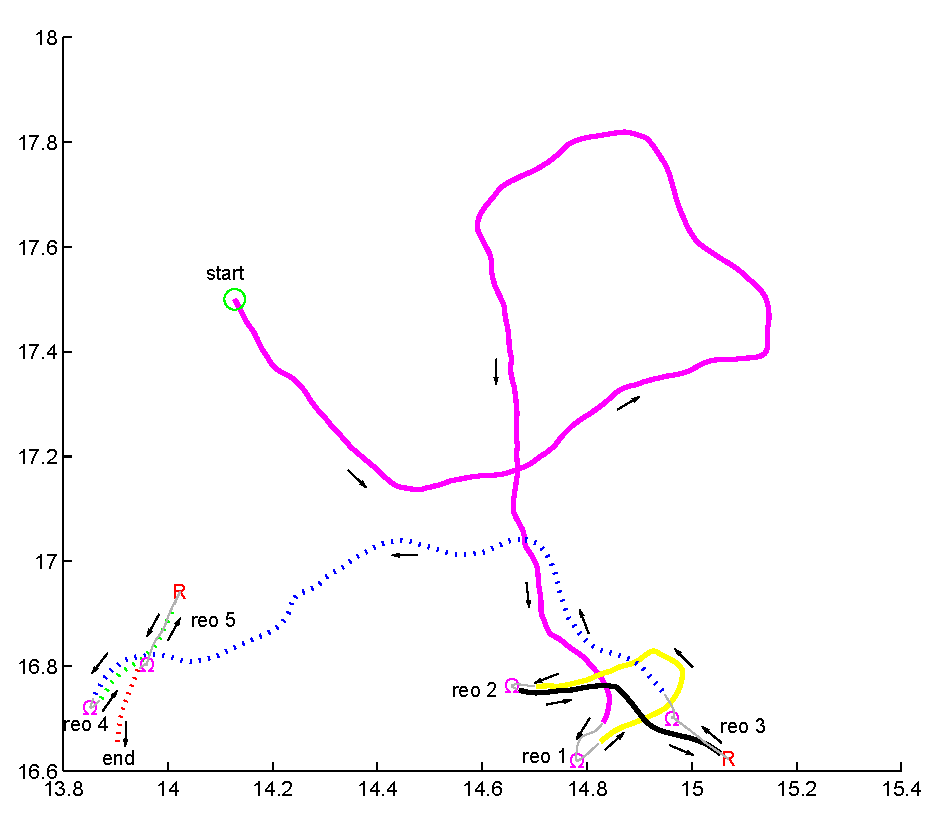
\includegraphics[width=6cm]{track3.eps}
%  (d)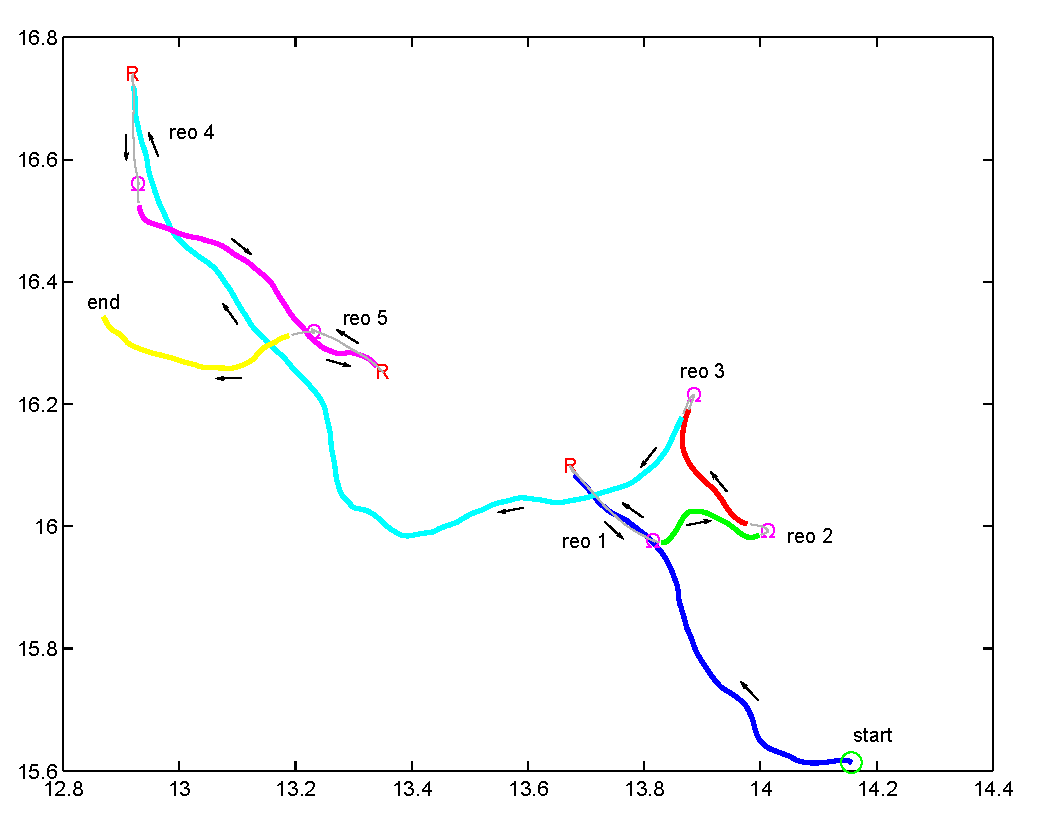
\includegraphics[width=6cm]{track4.eps}
%  %\input{.TpX}
%  \caption{Example tracks. Runs: Coloured, thin lines, reorientations: black, thin lines. Omega turns and reversals labelled as $\Omega$ and $R$. Grouping of turns into reorientations indicated by reo 1, reo 2, etc.} \label{fig:tracks}
%\end{figure}

\begin{figure}
  (a)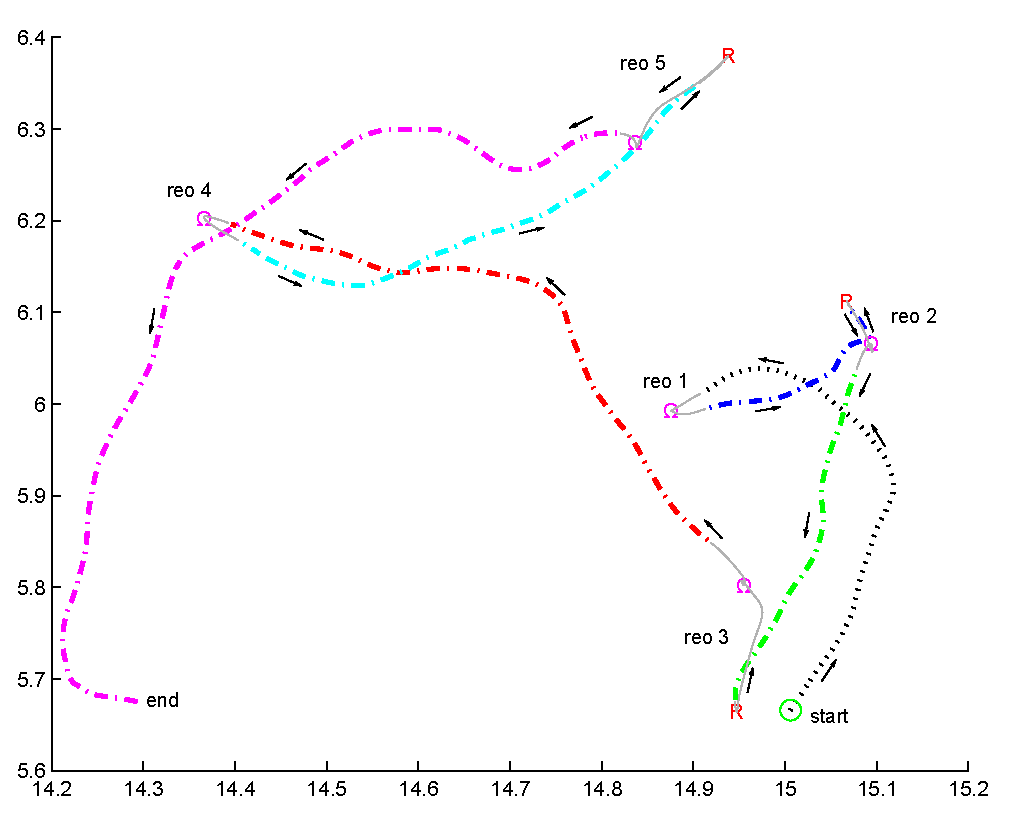
\includegraphics[width=6cm]{track2.eps}
  (b)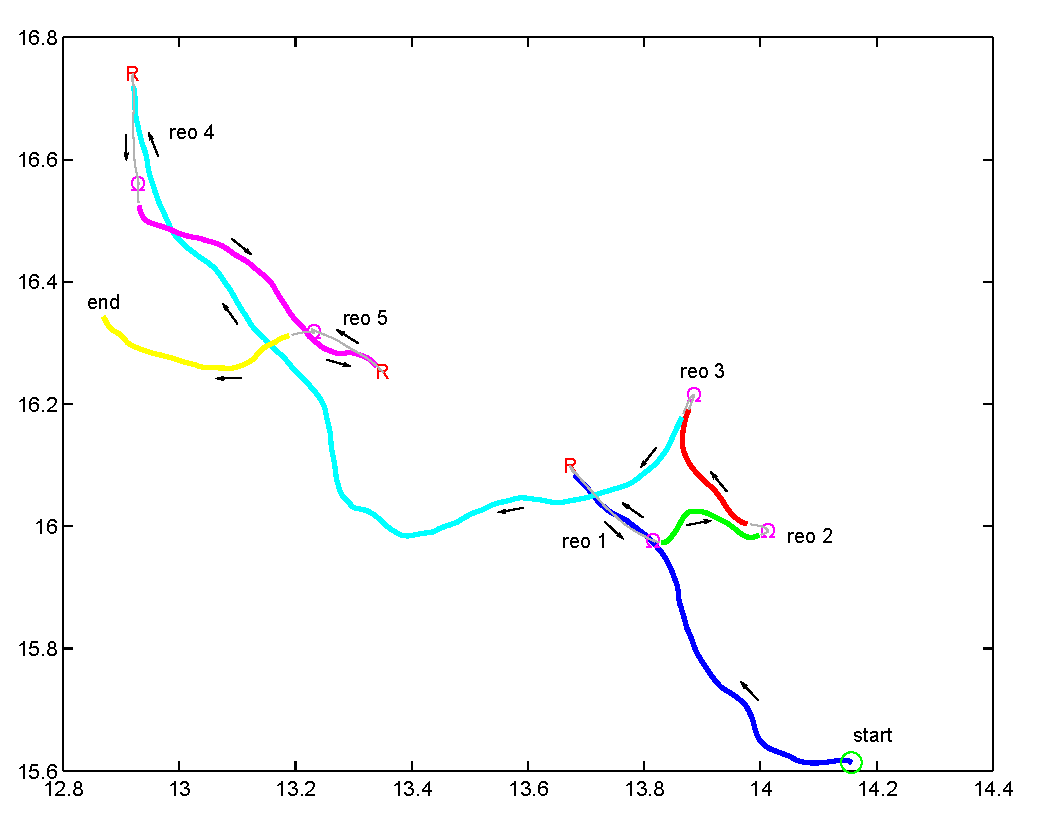
\includegraphics[width=6cm]{track4.eps}\\[1cm]
  (c)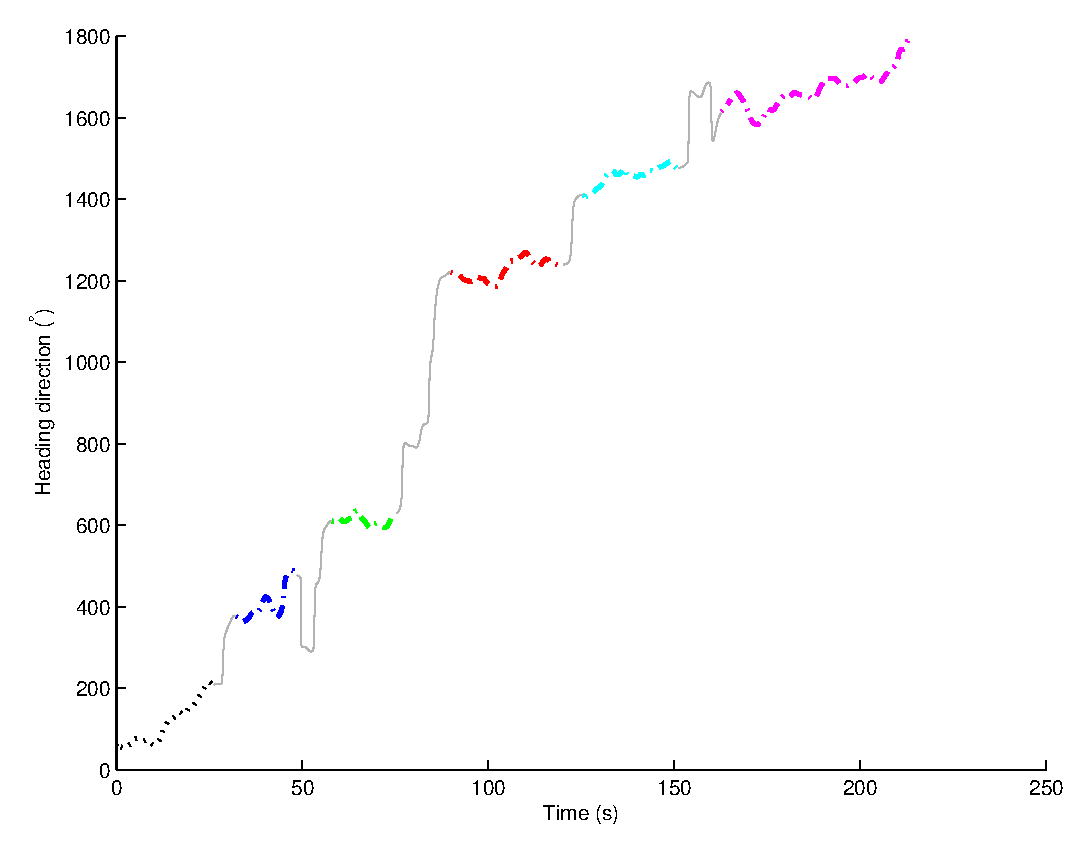
\includegraphics[width=6cm]{track2_dir.eps}
  (d)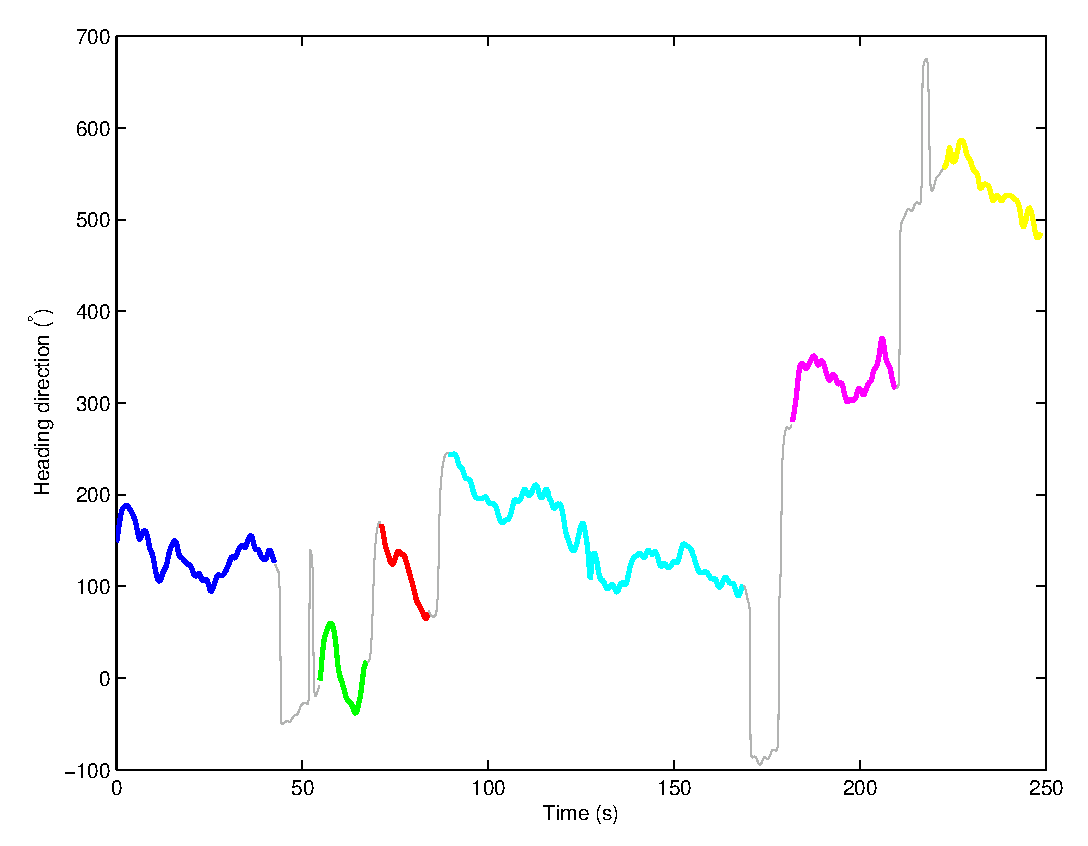
\includegraphics[width=6cm]{track4_dir.eps}\\[1cm]
  (e)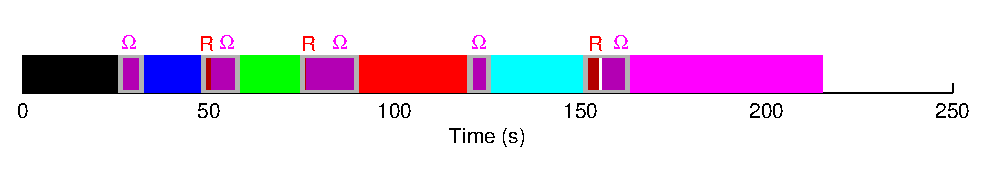
\includegraphics[width=6cm]{track2_type.eps}
  (f)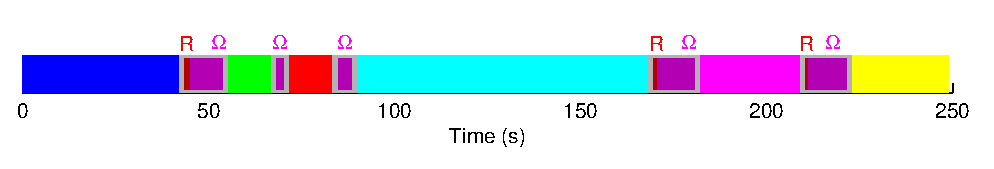
\includegraphics[width=6cm]{track4_type.eps}
  %\input{.TpX}
  \caption[Example tracks.]{(a-b)Example tracks. Runs: Coloured, thin lines, reorientations: black, thin lines. Omega turns and reversals labelled as $\Omega$ and $R$. Grouping of turns into reorientations indicated by reo 1, reo 2, etc.
  (c-d) heading direction during tracks in (a-b).
  (e-f) Segmentation into runs and turns.  } \label{fig:tracks}
\end{figure}



\begin{figure}
  \begin{center}
    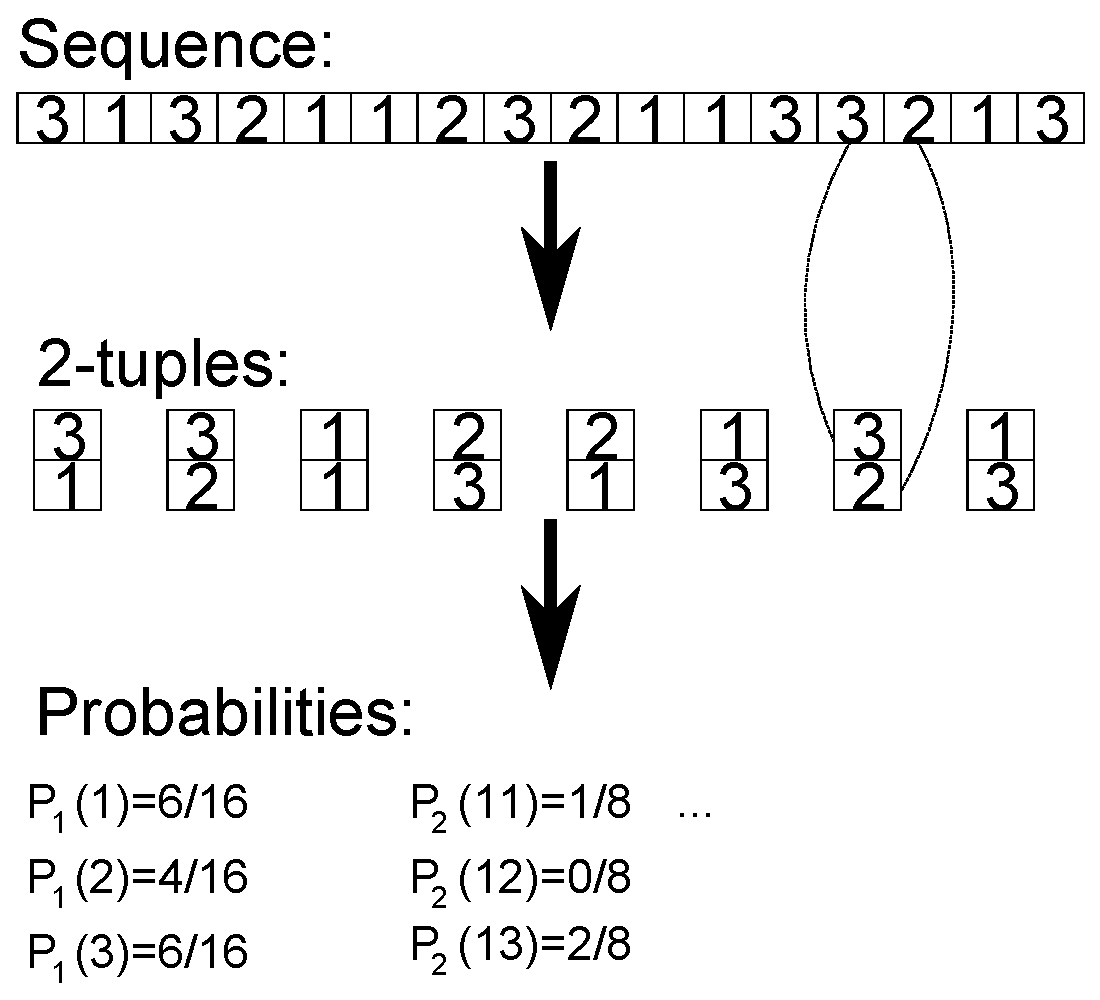
\includegraphics[width=10cm]{schematic.eps}
  \end{center}
  %\input{.TpX}
  \caption[Schematic calculation of probabilities.]{Schematic calculation of probabilities. (a) Sample sequence of reorientations. (b) Grouping sequence into $r$-tuples ($r=2$). (c) Estimating probabilities for individual members and for $r$-tuples from relative frequencies in sample.} \label{fig:schematic}
\end{figure}

In principle we should look at all the characteristics together. However, increasing the dimensionality of the data at each reorientation increases the number of bins used, which in turn increases the number of samples needed. Therefore, we will have to be satisfied with looking at each characteristic separately.

Note that this method can confuse animal-to-animal variability with causation. \Eg suppose that one of the worms makes larger turns than the others. In this situation, if the first reorientation in an $r$-tuple is large it would make it more likely that the worm in question is the large-turning one, making it more likely that the other reorientations in the $r$-tuple are large. Thus the probability distributions would not show independence even in the absence of actual causation. We will discuss the effect of animal-to-animal variability quantitatively in \sref{sec:variability} and show how to measure the amount of variability in \sref{sec:variest} and appendix \ref{sec:varibias}. The same thing applies to lack of stationarity. If runs tend to get longer over time, the same issue will arise.


\section{Entropy and mutual information}\label{sec:entropy}

The \textbf{entropy} of a probability distribution is a measure of the lack of information we have about a random variable \cite{Cover:2006}:
%
\begin{equation}\label{eq:ent}
  H(X) = \av{-\log P(X)}.
\end{equation}
%
It takes its minimum value of $0$ when $X$ can only take one value. It takes its maximum value of $\log n$ when $X$ has a uniform distribution over $n$ possibilities.

With several random variables, we can define a joint entropy from their joint probability distribution:
%
\begin{equation}\label{eq:jointent}
  H(X_1,\ldots,X_r) = \av{-\log P(X_1,\ldots,X_r)}.
\end{equation}
%
It satisfies the bounds
%
\begin{equation}\label{eq:entbounds}
  \max_i H(X_i) \leq H(X_1,\ldots,X_r) \leq \sum_{i=1}^r H(X_i).
\end{equation}
%
The lower bound is saturated when one of the variables is enough to determine the others, but it only makes sense for discrete distributions. The upper bound is saturated when the $X_i$ are independent:
%
\begin{equation}\label{eq:indent}
  P(X_1,\ldots,X_r) = \prod_{i=1}^r P(X_i)
  \quad \implies \quad
  H(X_1,\ldots,X_r) = \sum_{i=1}^r H(X_i).
\end{equation}
%

We can define the following measure of (lack of) independence:
%
\begin{equation}\label{eq:mutinf}
  I(X_1,\ldots,X_r) = \sum_{i=1}^r H(X_i) - H(X_1,\ldots,X_r) = \av{ \log \frac{P(X_1,\ldots,X_r)}{P(X_1)\ldots P(X_r)} }.
\end{equation}
%
In the case $r=2$, this is the \textbf{mutual information} between $X_1$ and $X_2$. For $r>2$, there are many different generalisations of mutual information. This one is called the \textbf{total correlation} \cite{Watanabe:1960}, or multiinformation. It has the properties:
%
\begin{itemize}
  \item it vanishes if and only if the random variables are independent
  \item otherwise, it is positive.
  \item it is bounded from above by $\sum_{i=1}^r H(X_i) - \max_i H(X_i)$.
\end{itemize}
%
We can define a normalised total correlation:
%
\begin{equation}\label{eq:normmutinfgen}
  C_r = \frac{I_r}{\sum_{i=1}^r H(X_i) - \max_i H(X_i)}, \qquad 0 \leq C_r \leq 1.
\end{equation}
%
The lower bound corresponds to complete independence. The upper bound corresponds to complete redundancy.

In our cases, the random variables, $X_i$, all have the same marginal distribution, so $H(X_i)=H_1\; \forall i$ and the total correlation satisfies the bounds
%
\begin{equation}\label{eq:mutinfbounds}
  0 \leq I_r(X_1,\ldots,X_r) \leq (r-1)H_1.
\end{equation}
%
and the normalised version is:
%
\begin{equation}\label{eq:normmutinf}
  C_r = \frac{I_r}{(r-1)H_1}, \qquad 0 \leq C_r \leq 1.
\end{equation}
%
We will use this version except where explicitly stated otherwise.

\subsection{Entropy, information and bits}\label{sec:bits}

If we take the logarithms to base 2, we can think of entropy as a measure of ``the average number of bits'' of information we are missing by not knowing the value of $X$, and hence the number of bits of information we'd gain by measuring it. \Eg suppose $X$ can take on two values with equal probability, then $H(X)=1$. If the probabilities were 1 and 0, then $H(X)=$, as we'd gain no information by measuring it due to the fact that we already know its value. If we have $n$ independent two state systems of the first type, we'd have an entropy of $n$ due to \eqref{eq:indent}. On the other hand, if the first bit determined the remaining $n-1$ bits, we'd have an entropy of 1.

There is another way of thinking of mutual information in terms of \textbf{conditional entropy}:
%
\begin{equation}\label{eq:condent}
  H(Y|X) = \av{-\log P(Y|X)},
\end{equation}
%
where the average is over all values of $X$ and $Y$. This can be thought of as the number of bits of missing information due to not knowing $Y$ that remain after measuring $X$.

Then the mutual information can be written as
%
\begin{equation}\label{eq:mutinfcond}
  I(X,Y) = H(Y) - H(Y|X) = H(X) - H(X|Y),
\end{equation}
%
\ie it is the number of bits of information about $Y$ that we gain by measuring $X$ (and vice-versa).

When we have three random variables, we can write
%
\begin{equation}\label{eq:multiinfcond3}
  \begin{aligned}
    I_3 &= \av{\log \frac{P(X_1,X_2,X_3)}{P(X_1)P(X_2)P(X_3)}} \\
      &=  \av{\log \frac{P(X_2 \vert X_1)}{P(X_2)}} + \av{\log \frac{P(X_3 \vert X_1,X_2)}{P(X_3)}} \\
      &= \brk{H(X_2)-H(X_2|X_1)} +  \brk{ H(X_3)-H(X_3|X_1,X_2)}.
  \end{aligned}
\end{equation}
%
In general, we can write
%
\begin{equation}\label{eq:multiinfcondgen}
  \begin{aligned}
    I_r &= \av{\log \frac{P(X_1,X_2,\ldots,X_r)}{P(X_1)P(X_2)\ldots P(X_r)}} \\
      &=  \av{\log \frac{P(X_2 \vert X_1)}{P(X_2)}} +\ldots+ \av{\log \frac{P(X_r \vert X_1,\ldots,X_{r-1})}{P(X_r)}} \\
      &= \brk{H(X_2)-H(X_2|X_1)} + \ldots + \brk{ H(X_r)-H(X_r|X_1,\ldots,X_{r-1})} \\
      &= \sum_{i=2}^{r} \brk{ H(X_i)-H(X_i|X_1,\ldots,X_{i-1})}.
  \end{aligned}
\end{equation}
%
\ie its the sum of number of bits of information about each $X_i$ that we gain by measuring the previous ones.


\subsection{Markov processes}\label{sec:markov}

If the process is Markovian (in the discrete sense), \ie one reorientation/run is only affected by the previous reorientation/run and not any earlier ones, then $P(X_3 \vert X_1,X_2)$ is independent of $X_1$, and is the same function as $P(X_2 \vert X_1)$. Therefore
%
\begin{equation}\label{eq:tripvspair}
  \begin{aligned}
    H(X_3|X_1,X_2) &= H(X_2|X_1).\\
    I_3 &= 2I_2, \qquad C_3 = \frac{I_3}{2H_1} = C_2.
  \end{aligned}
\end{equation}
%
Similar arguments apply for longer $r$-tuples:
 %
 \begin{equation}\label{eq:markovinf}
   I_r = (r-1)I_2, \qquad C_r = \frac{I_r}{(r-1)H_1} = C_2.
\end{equation}
%
One can look for non-Markovian behaviour by looking for differences in $C_r$ for different $r$.


\subsection{Effect of animal-to-animal variability}\label{sec:variability}

In this section we will look at the effect that animal-to-animal variability can have on mutual information in the case of binary output, \ie the characteristics of each reorientation are reduced to two possible outcomes which we will call $\{+,-\}$. In specific cases these two outcomes will be the two most important reorientation types (omega or reversal-omega) and the reorientation direction (right or left). We will assume that animal-to-animal variability is the only effect and that there is no memory

Label the individual worms with $i=1\ldots N$. Then, for a single reorientation
%
\begin{equation}\label{eq:varisinglereo}
  P(i) = q_i, \qquad
  P(+|i) = p_i, \qquad
  P(-|i) = 1-p_i.
\end{equation}
%
The prior probability that a reorientation was from a particular animal, $q_i$, will be proportional to that animal's reorientation rate, which may not be the same for all animals. We also introduce the notation
%
\begin{equation}\label{eq:varinot}
  \bar{p} = \sum_i q_i p_i, \qquad
  \sigma_p = \sqrt{\sum_i q_i(p_i-\bar{p})^2}.
\end{equation}
%
So that
%
\begin{equation}\label{eq:varimarg}
  P(+) = \bar{p}, \qquad P(-) = 1-\bar{p}.
\end{equation}
%
Then, using Bayes' theorem
%
\begin{equation}\label{eq:singlereobayes}
  P(i|+) = \frac{P(+|i)P(i)}{P(+)} = \frac{q_ip_i}{\bar{p}}, \qquad
  P(i|-) = \frac{P(-|i)P(i)}{P(-)} = \frac{q_i(1-p_i)}{1-\bar{p}}.
\end{equation}
%

For pairs of successive reorientations, we use the notation
%
\begin{equation}\label{eq:varipairnot}
  P(\text{next}=a|\text{prev}=b) = P(a|b) , \qquad
  P(\text{prev}=b \cap \text{next}=a) = P(b,a) .
\end{equation}
%
We can calculate conditional probabilities for next reorientation, given previous reorientation
%
\begin{equation}\label{eq:varicond}
  \begin{aligned}
    P(+|+) &= \sum_i P(+|i)P(i|+) = \bar{p} + \frac{\sigma_p^2}{\bar{p}}, \\
    P(+|-) &= \sum_i P(+|i)P(i|-) = \bar{p} - \frac{\sigma_p^2}{1-\bar{p}}, \\
    P(-|+) &= \sum_i P(-|i)P(i|+) = 1-\bar{p} - \frac{\sigma_p^2}{\bar{p}}, \\
    P(-|-) &= \sum_i P(-|i)P(i|-) =1- \bar{p} + \frac{\sigma_p^2}{1-\bar{p}},
  \end{aligned}
\end{equation}
%
and the joint probabilities of previous and next reorientations
%
\begin{equation}\label{eq:varijoint}
  \begin{aligned}
    P(+,+) &= P(+|+)P(+) = \bar{p}^2 + \sigma_p^2, \\
    P(+,-) &= P(-|+)P(+) = \bar{p}(1-\bar{p}) - \sigma_p^2, \\
    P(-,+) &= P(+|-)P(-) = \bar{p}(1-\bar{p}) - \sigma_p^2, \\
    P(-,-) &= P(-|-)P(-) = (1-\bar{p})^2 + \sigma_p^2.
  \end{aligned}
\end{equation}
%

The entropy of single reorientations is then
%
\begin{equation}\label{eq:varient}
  H_1 = - \sum_{a\in\{+,-\}} P(a)\log P(a)
   = - \bar{p}\log \bar{p} - (1-\bar{p})\log(1-\bar{p}),
\end{equation}
%
and the mutual information is
%
\begin{equation}\label{eq:varimutinf}
  \begin{aligned}
  I_2 =& \sum_{a,b\in\{+,-\}} P(a,b)\log \frac{P(a,b)}{P(a)P(b)}\\
   =& \prn{\bar{p}^2 + \sigma_p^2}\log\prn{1 + \frac{\sigma_p^2}{\bar{p}^2}}
   + 2\prn{\bar{p}(1-\bar{p}) - \sigma_p^2}\log\prn{1 - \frac{\sigma_p^2}{\bar{p}(1-\bar{p})}}
   \\&+ \prn{(1-\bar{p})^2 + \sigma_p^2}\log\prn{1 + \frac{\sigma_p^2}{(1-\bar{p})^2}},
  \end{aligned}
\end{equation}
%
which vanishes when $\sigma_p=0$.


\section{Practical issues}\label{sec:practical}

\subsection{Correcting systematic errors in entropy and mutual information}\label{sec:syscorr}

We will compute the quantities defined in the previous section by estimating the probability distributions, $P_1(X_i)$ and $P_r(X_1,\ldots,X_r)$ from the relative frequencies in sample sequences of reorientations. As all the $X_i$ have the same marginal distribution, we will estimate $P_1(X)$ from the pooled data, rather that estimating the $P_1(X_i)$ separately.


The lower bounds on mutual information, \eqref{eq:mutinfbounds} and \eqref{eq:normmutinf}, lead to systematic errors which tend to bias these estimates upwards. There are several methods for estimating this bias.

One approach involves expending the errors in the reciprocal of the sample size and estimating the leading order correction, see \cite{Roulston1999}. One can also estimate the random errors using this approach. Our estimators are slightly different to those used there, the appropriate versions of the estimates are calculated in Appendix \ref{sec:stderr}.

As the bias estimates are independent of the actual probability distribution, depending only on sample size and number of bins, we can estimate the bias by computing the mutual information for a completely random sequence in the same way. As the true value is zero, the result of this computation is an estimate of the bias. Furthermore, if the probabilities of the individual elements of the sequence are the same as in the data, this can be regarded as a Monte-Carlo simulation of the null hypothesis -- that the individual elements of the sequence are independent of each other. Thus, we can compute a p-value by seeing where the original result ranks amongst the results of the simulation.

We will do this using the non-parametric bootstrap. This is conceptually similar to the common alternative procedure of shuffling the sequence. Shuffling can be thought of as resampling without replacement, whereas the non-parametric bootstrap is resampling with replacement. They both involve removing any information in the sequence without changing the probabilities of the individual elements.

The direct method of \cite{Strong1998} consists of varying the sample size and extrapolating to infinity. This can also be used to check that the number of samples is large enough compared to the number of bins. With this method, it is difficult to compute error bars and p-values, as the process is slow.

We show three examples of these methods in \fref{fig:biascomp}, one where they agreed really well, one where the agreement was not too bad and one where it was terrible. In the last case, it even showed the wrong trend: the bias is supposed to be positive and decreasing with increasing sample size. This probably indicates that the sample size is too small and we were not in the asymptotic regime where the results of appendix \ref{sec:stderr} can be trusted.

We can see how much this discrepancy varied with sample size in \fref{fig:discrep}. This can be used as a guide for when $N$ is large enough to trust the results.


\begin{figure}
  \begin{center}
    (a)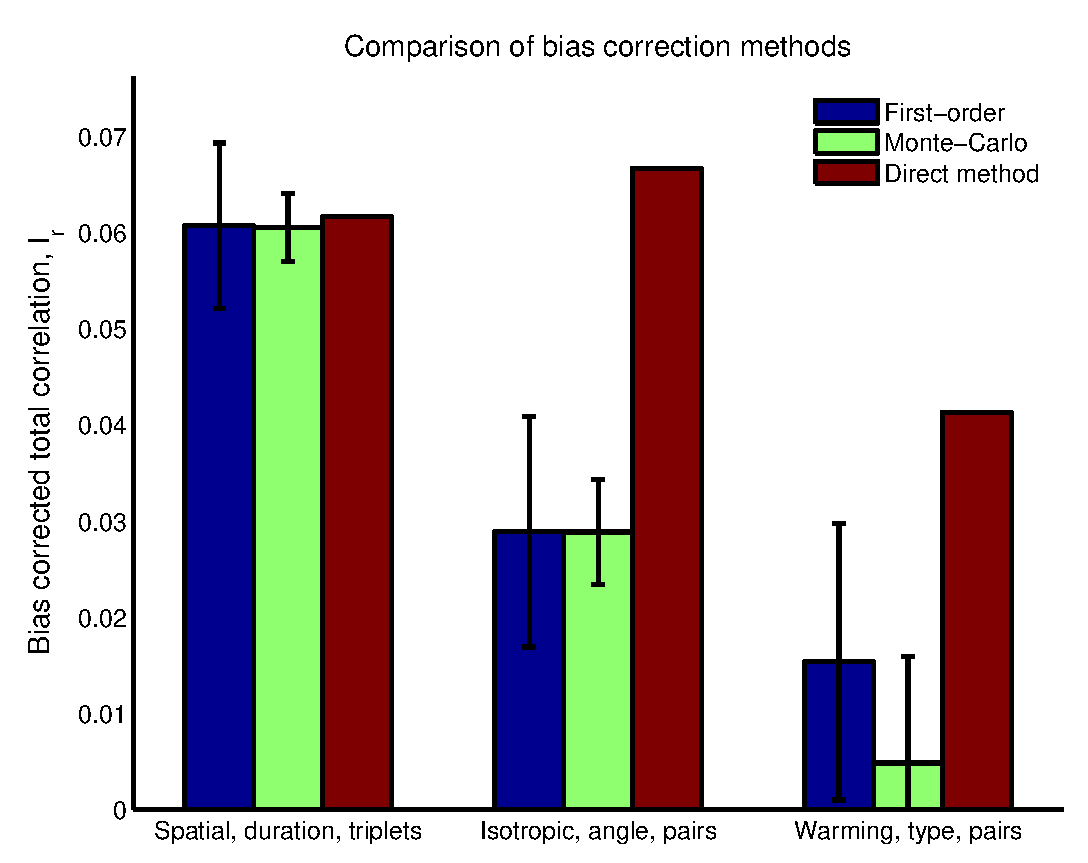
\includegraphics[width=7cm]{comparison.eps}
    (b)i)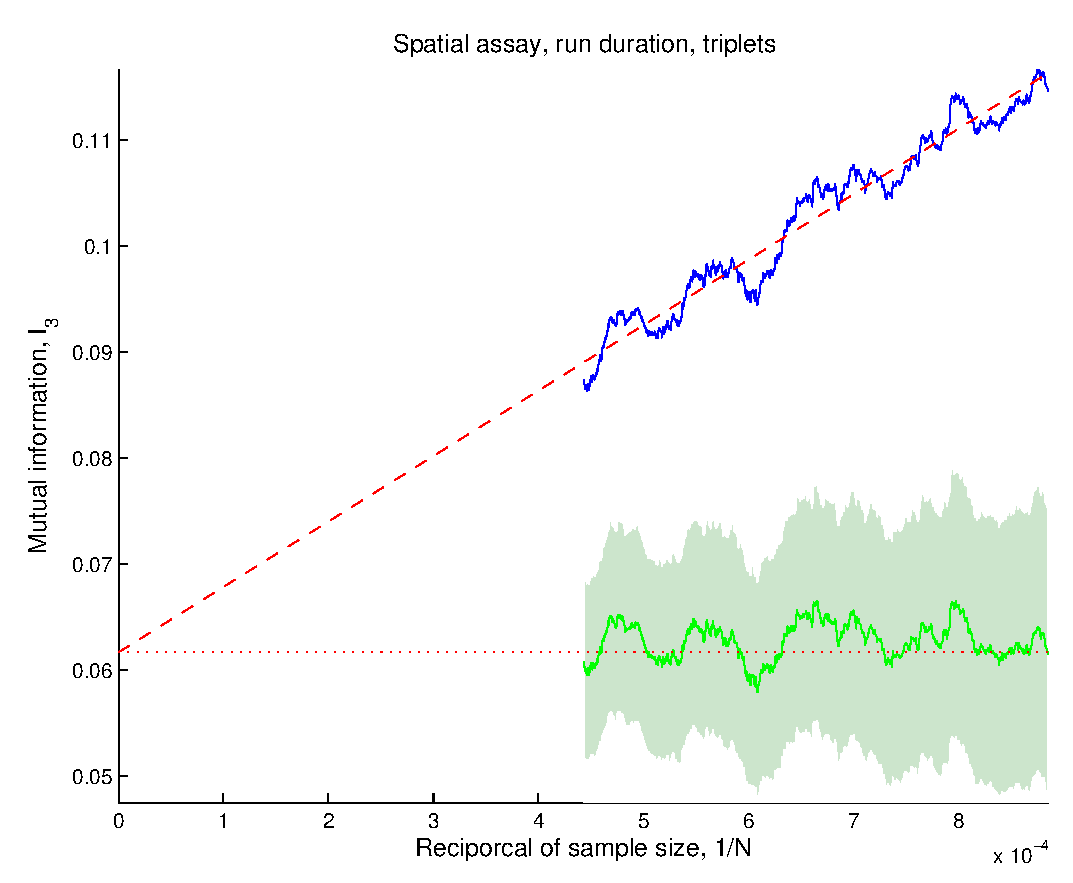
\includegraphics[width=7cm]{spat_dur_3.eps}\\
    ii)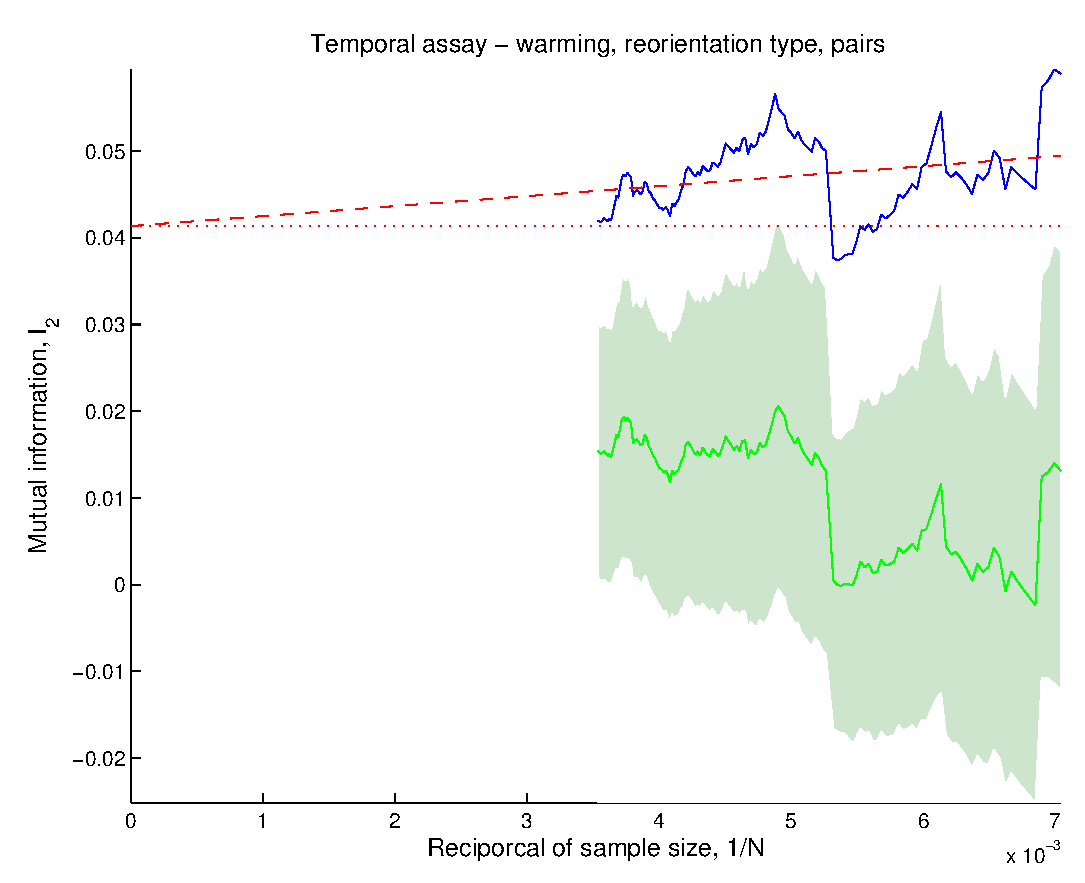
\includegraphics[width=7cm]{warm_typ_2.eps}
    iii)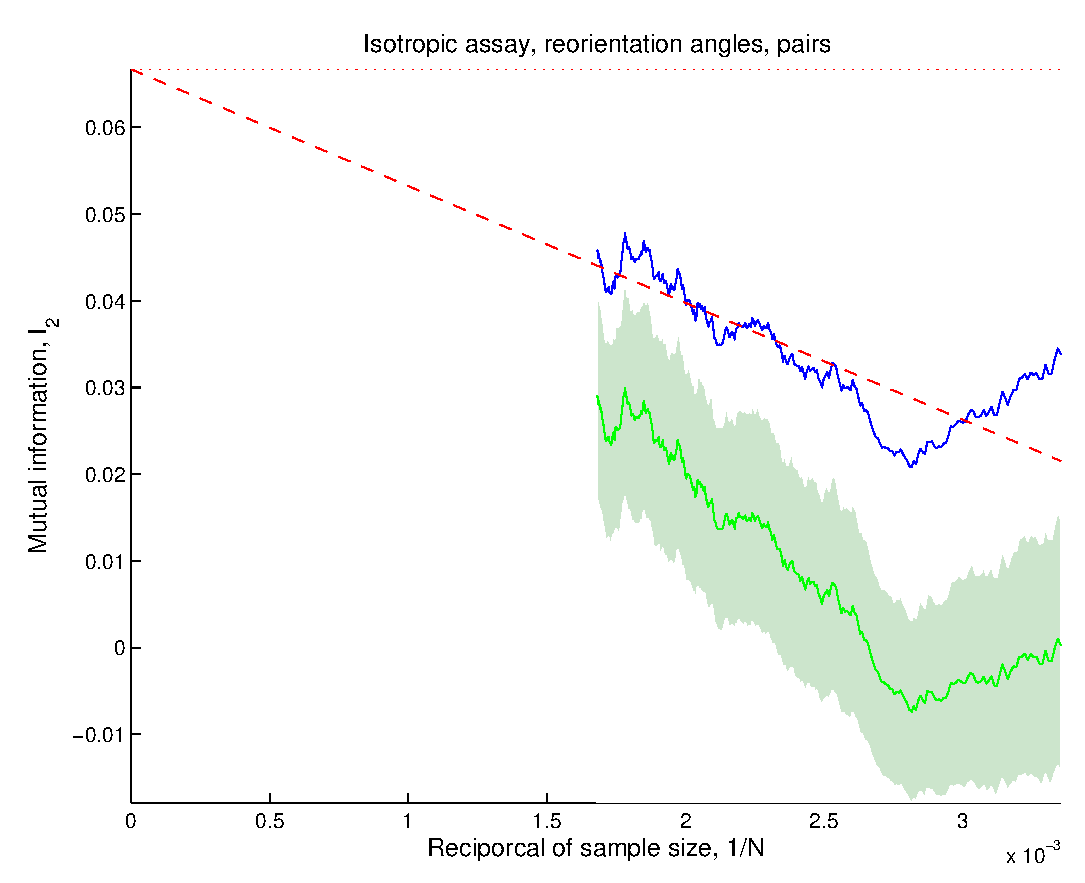
\includegraphics[width=7cm]{iso_ang_2.eps}
  \end{center}
  \caption[Comparison of different methods for removing bias.]{Comparison of different methods for removing bias. (a) Three examples of the three unbiased estimates of mutual information/total correlation. First-order refers to the methods of appendix \ref{sec:stderr}. Monte-Carlo refers to subtracting the mean of 1000 nonparametric bootstrap simulations, the error-bars are the standard deviation of the bootstrap simulations. (b) Illustration of the direct method, Blue line is the uncorrected estimates with different sample sizes, red dashed line shows the extrapolation to infinite sample size and red dotted line indicates the result of this extrapolation. Green line shows the unbiased estimator using the first-order method of appendix \ref{sec:stderr} for comparison, darker green shading is $\pm$ one standard error. i)-iii) the three cases shown in (a).} \label{fig:biascomp}
\end{figure}

\begin{figure}
  \begin{center}
    (a)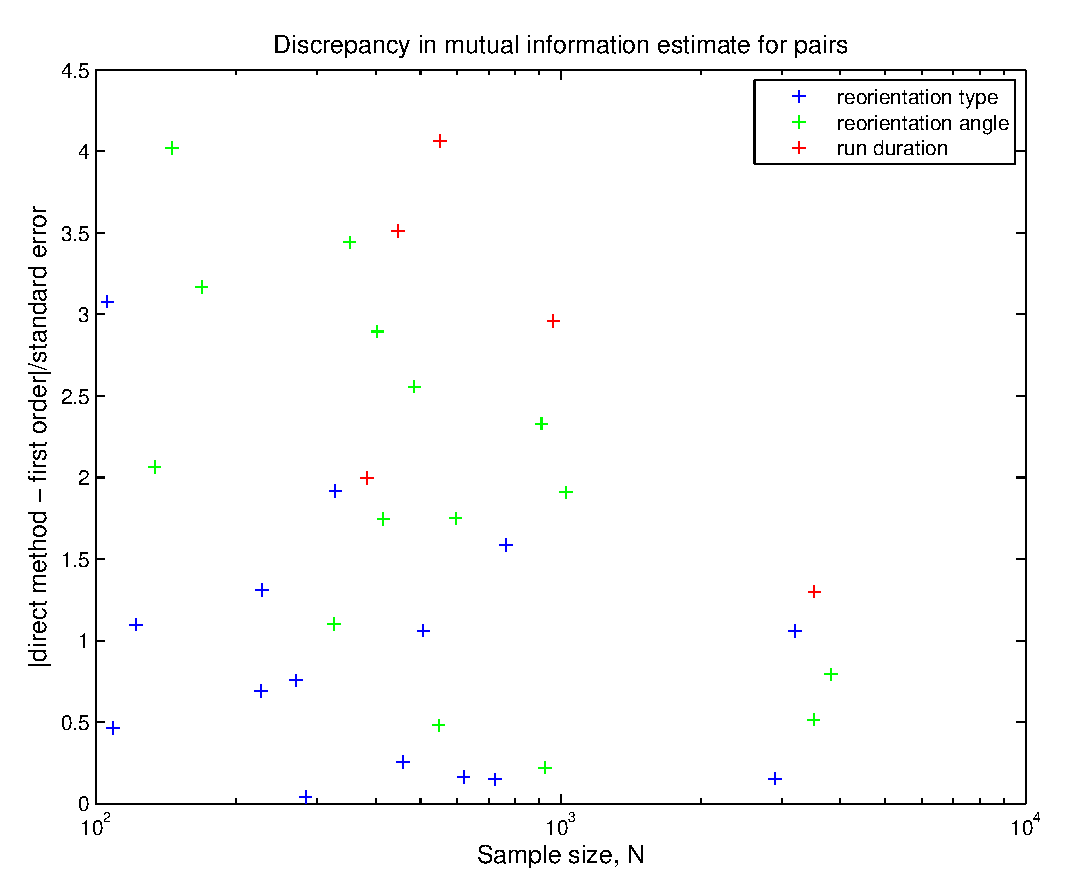
\includegraphics[width=7cm]{discpair.eps}
    (b)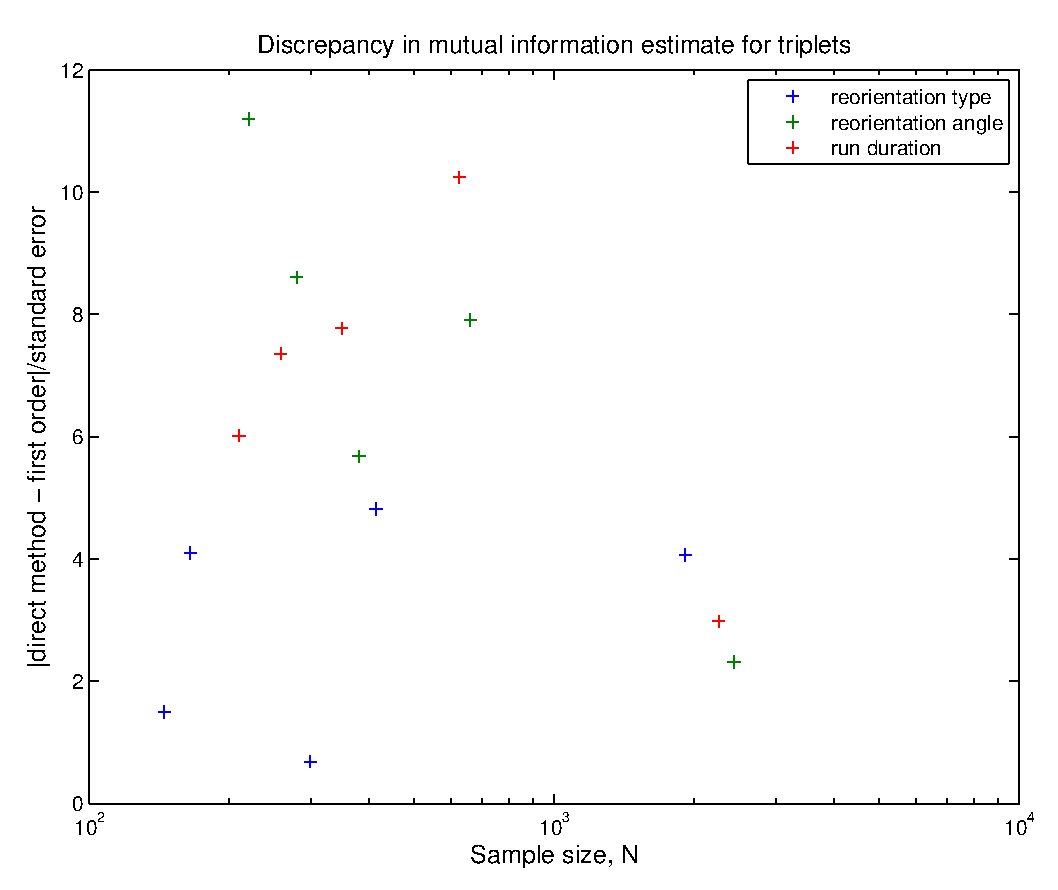
\includegraphics[width=7cm]{disctrip.eps}
  \end{center}
  \caption[Effect of sample size in discrepancy between bias removal methods.]{Effect of sample size in discrepancy between bias removal methods; size of discrepancy between unbiased estimates from direct method and first order method divided by first order standard error for (a) pairs (maximum of 25 bins) (b) triplets (maximum of 125 bins).} \label{fig:discrep}
\end{figure}


\subsection{Estimating animal-to-animal variability}\label{sec:variest}

Estimating $\sigma_p$ in \eqref{eq:varinot} is tricky, as we can't keep track of animal identity during collisions (a problem that does not affect $\bar{p}$, see \eqref{eq:variests} below). What we will do is to restrict attention to those tracks that start during the first $20\mins$ and are at least $20\mins$ long. This ensures that each animal is sampled at most once and that we have a decent amount of data for each animal. We also only consider the first $20\mins$ of each track (whilst this reduces the amount of data, it makes it possible to estimate bias and standard error, see appendix \ref{sec:varibias}). We will then assume that the estimate for $\sigma_p$ applies to the whole experiment. Whilst the turning rates do change during the experiment, we only care about the ratio of turning rates between different animals, which we will assume remains constant.

For reorientation type, we count the number of omegas in each track, $\Omega_i$, and the number of reversal-omegas, $R_i$. If the track length is $t_i$,
%
\begin{equation}\label{eq:varesttype}
  \hat{n}_i = \Omega_i+R_i, \qquad
  N = \sum_i \hat{n}_i, \qquad
  \hat{q}_i = \frac{\hat{n}_i}{N}, \qquad
  \hat{p}_i = \frac{\Omega_i}{\Omega_i+R_i}.
\end{equation}
%

For reorientation direction, we count the number of right turns in each track, $R_i$, and the number of left turns, $L_i$. If the track length is $t_i$,
%
\begin{equation}\label{eq:varestdir}
  \hat{n}_i = \frac{R_i+L_i}{t_i}, \qquad
  N = \sum_i \hat{n}_i, \qquad
  \hat{q}_i = \frac{\hat{n}_i}{N}, \qquad
  \hat{p}_i = \frac{R_i}{R_i+L_i}.
\end{equation}
%

In both cases, $\bar{p}$ can be estimated by substituting \eqref{eq:varesttype} or \eqref{eq:varestdir} into \eqref{eq:varinot}. However, estimating $\sigma_p^2$ is more complicated, as the variance of the sample also receives contributions from the Binomial statistics of each track. In appendix \ref{sec:varibias}, we discuss the construction of approximately unbiased estimators and their variance. The result is
%
\begin{equation}\label{eq:variests}
  \begin{aligned}
    \hat{\bar{p}} &= \sum_i \hat{q}_i \hat{p}_i
       =\left\{\begin{aligned}
      & \frac{\sum_i \Omega_i}{N} \quad \text{for reorientation type,}\\
      & \frac{\sum_i R_i}{N}  \quad \text{for reorientation direction,}
       \end{aligned}\right. \\
    \var(\hat{\bar{p}}) &\approx \frac{\hat{\bar{p}}(1-\hat{\bar{p}})}{N}.,\\
    \hat{\sigma}_p^2 &= \frac{N+1}{N} \sum_i\prn{ \hat{q}_i(\hat{p}_i-\hat{\bar{p}})^2 - \frac{\hat{q}_i(1-\hat{q}_i)\hat{p}_i(1-\hat{p}_i)}{\hat{n}_i}}.
  \end{aligned}
\end{equation}
%
The expression for the variance of $\hat{\sigma}_p^2$ is a colossal mess. Instructions for computing it can be found in appendix \ref{sec:varibias}.

As the second expression for $\hat{\bar{p}}$ doesn't rely on maintaining animal identity, we can use the full data set to estimate it. As we will use a larger data set for $\hat{\bar{p}}$ than for $\hat{\sigma}_p^2$, we ignore possible correlations in their standard errors when computing standard errors in derived quantities.

The results of this analysis for worms without any stimulus is shown in \fref{fig:variability}. The p-values for seeing at least the spread that we get without any animal-to-animal variability are in table \ref{tab:varipval}.

\begin{figure}
  (a)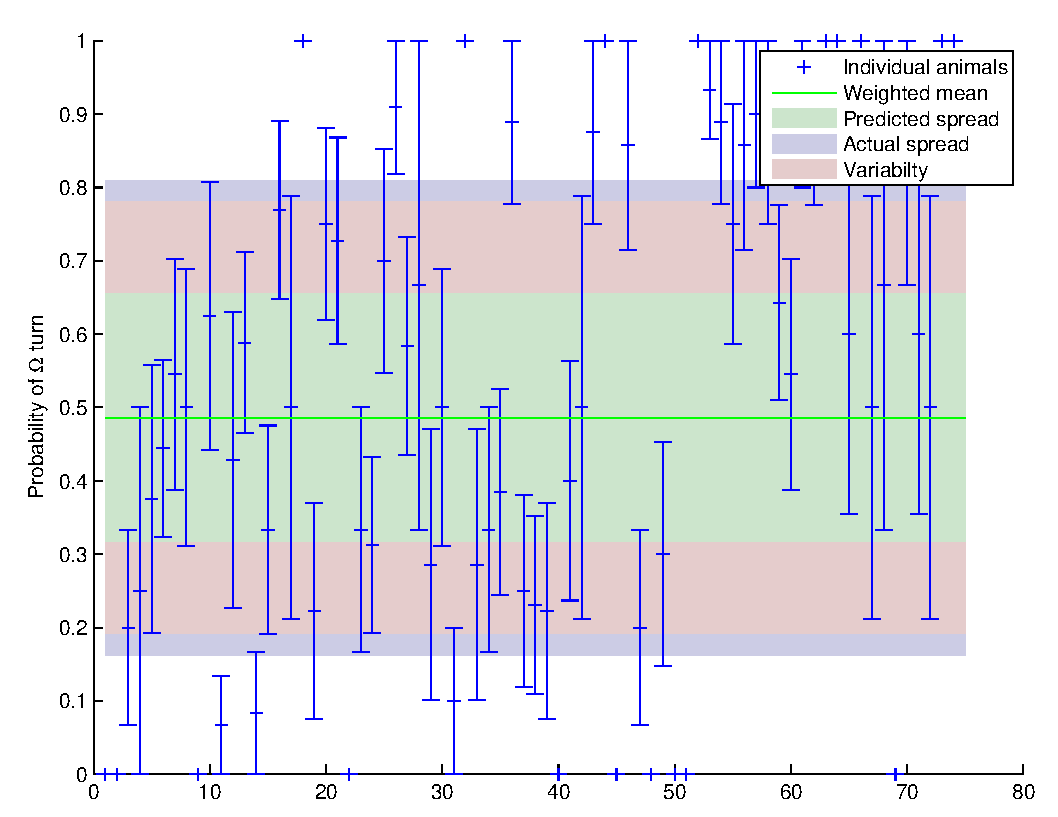
\includegraphics[width=7cm]{TypeProbs_individual.eps}
  (b)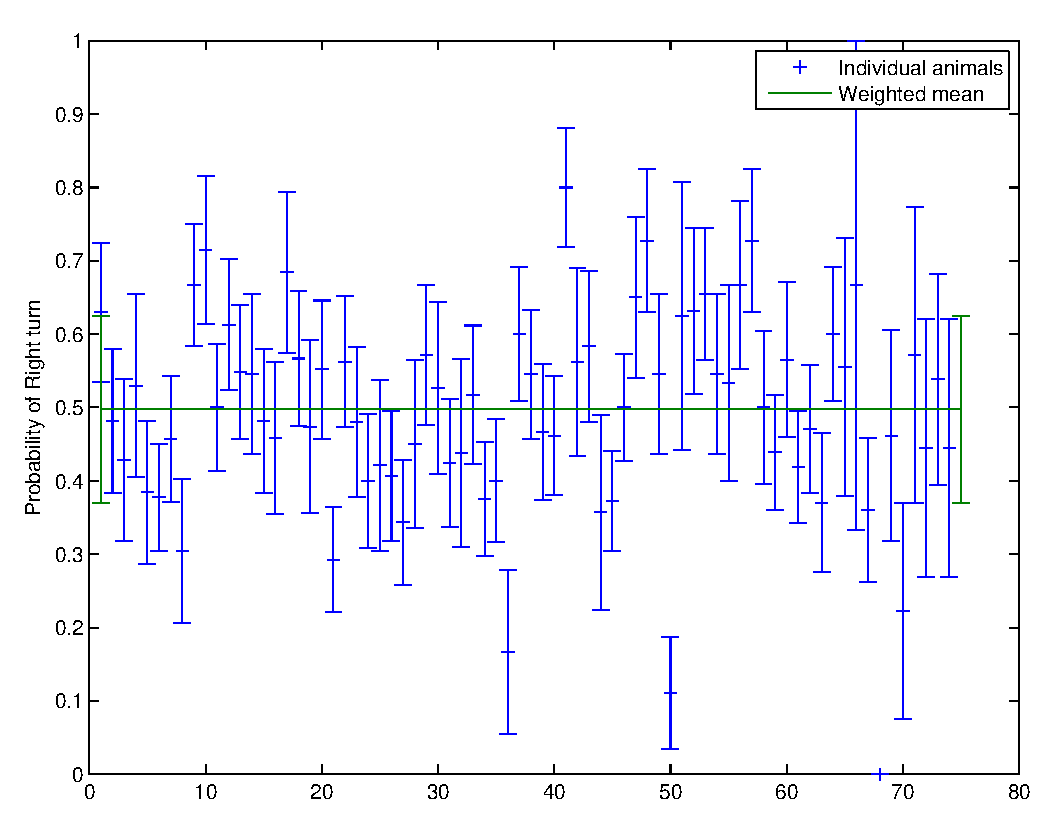
\includegraphics[width=7cm]{DirProbs_individual.eps}
  %\input{.TpX}
  \caption[Estimating animal-to animal variability.]{Estimating animal-to animal variability. (a) probability of $\Omega$ turns for individual animals and the weighted mean. (b) probability of Right turns for individual animals and the weighted mean. The weighted mean is $\hat{\bar{p}}$ \eqref{eq:variests}.
  The green shaded region is $\pm$ the standard deviation one would expect if each animal's number of reorientations was equal to the mean.
  The blue shaded region is $\pm$ the actual standard deviation observed (computed by substituting (\ref{eq:varesttype}) or (\ref{eq:varestdir}) into (\ref{eq:varinot})).
  The red shaded region is $\pm$ the amount of animal-to-animal variability needed to explain the difference, $\hat{\sigma}_p$ \eqref{eq:variests}. }\label{fig:variability}
\end{figure}

\begin{table}
  \begin{center}
    \begin{tabular}{|r|l|l|}
      \hline
      % after \\: \hline or \cline{col1-col2} \cline{col3-col4} ...
      Assay & Type & Direction \\
    \hline
     Neutral      & $1\ee{-24}$ & $0.02$  \\
     Cryophilic   & $6\ee{-11}$ & $3\ee{-4}$  \\
     Thermophilic & $2\ee{-19}$ & $7\ee{-7}$ \\
     Saltphilic   & $2\ee{-29}$ & $4\ee{-5}$ \\
     Saltphobic   & $7\ee{-54}$ & $5\ee{-12}$ \\
     \hline
    \end{tabular}
%    \begin{tabular}{|r|l|l|}
%      \hline
%      % after \\: \hline or \cline{col1-col2} \cline{col3-col4} ...
%      Assay & Type & Direction \\
%    \hline
%     Neutral      & $0$ & $0.02$  \\
%     Cryophilic   & $4\ee{-14}$ & $3\ee{-4}$  \\
%     Thermophilic & $0$ & $9\ee{-7}$ \\
%     Saltphilic   & $0$ & $5\ee{-5}$ \\
%     Saltphobic   & $0$ & $6\ee{-12}$ \\
%     \hline
%    \end{tabular}
  \end{center}
  \caption[P-values for variability]{P-values for variability, \ie the likelihood of observing at least the spread seen in \fref{fig:variability} assuming no animal-to-animal variability. Computed with a $\chi^2$ test, \ie the binomial distribution was approximated by a Gaussian.}\label{tab:varipval}
\end{table}



\section{Results}\label{sec:results}


\subsection{Binary cases}\label{sec:binaryresults}

Now we will restrict attention to binary cases, \ie when looking at reorientation types, we will restrict attention to the 2 most common types - \emph{omega} and \emph{reversal-omega} (the probabilities of the different types are shown in \fref{fig:typeprob}). For reorientation angle we only pay attention to the sign, \ie whether it is to the right or to the left.

The analysis was performed for isotropic assays (where the temperature was held uniform and constant at $20\dC$) and spatial assays (where the temperature was constant in time but varied linearly in space from $18-23\dC$ over $22\cm$). These were done with worms cultivated at $20\dC$ (neutral), $15\dC$ (cryophilic) ant $25\dC$ (thermophilic). It was also done for worms grown on $50\mM$ salt concentration on a spatial salt gradient from $0-50\mM$ over $22\cm$ (saltphilic) and on a gradient from $50-100\mM$ also over $22\cm$ (saltphobic).

We only looked at the cases $r=2$ (pairs of consecutive reorientations). The results are in \fref{fig:binaryresults}. The p-values for differences in conditional probabilities can be found in table \ref{tab:condpval}.


\begin{figure}
  \begin{center}
    (a)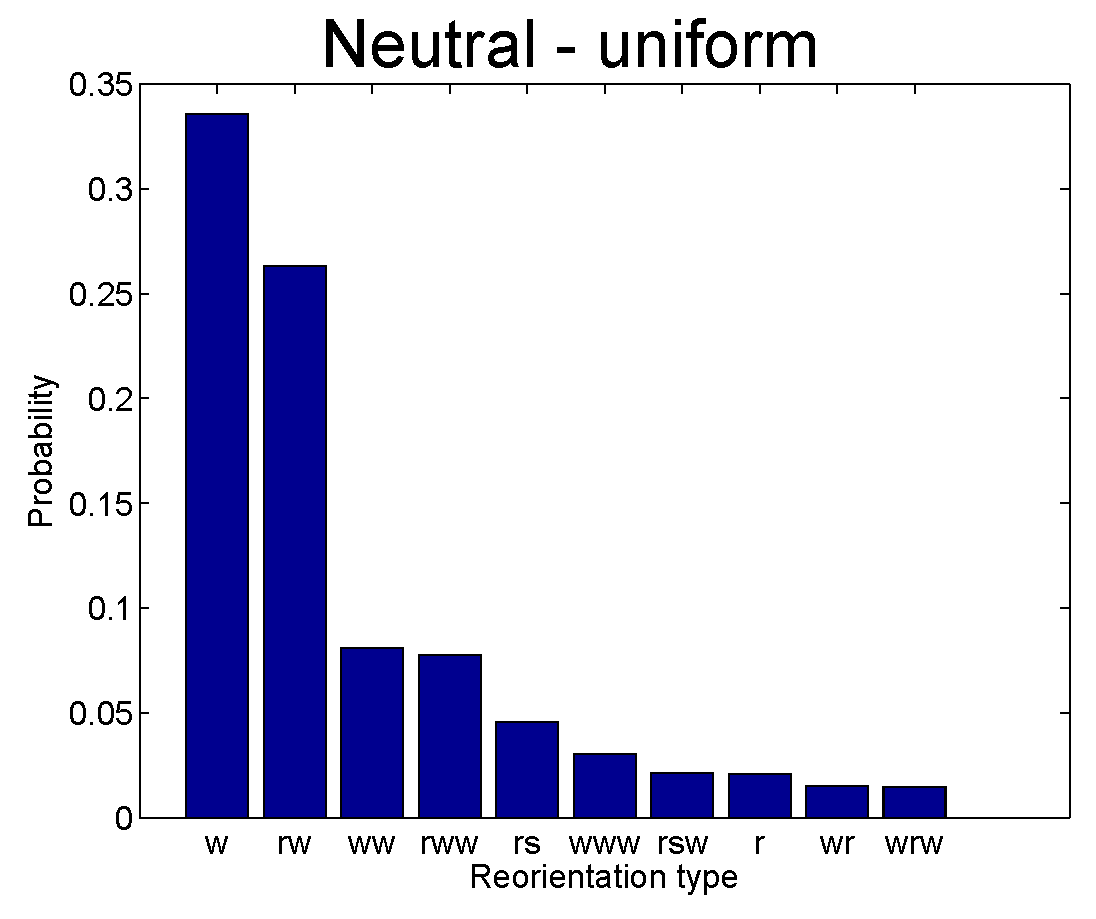
\includegraphics[width=6cm]{ReoTypeProb-neutraliso.eps}\\[1cm]
    (b)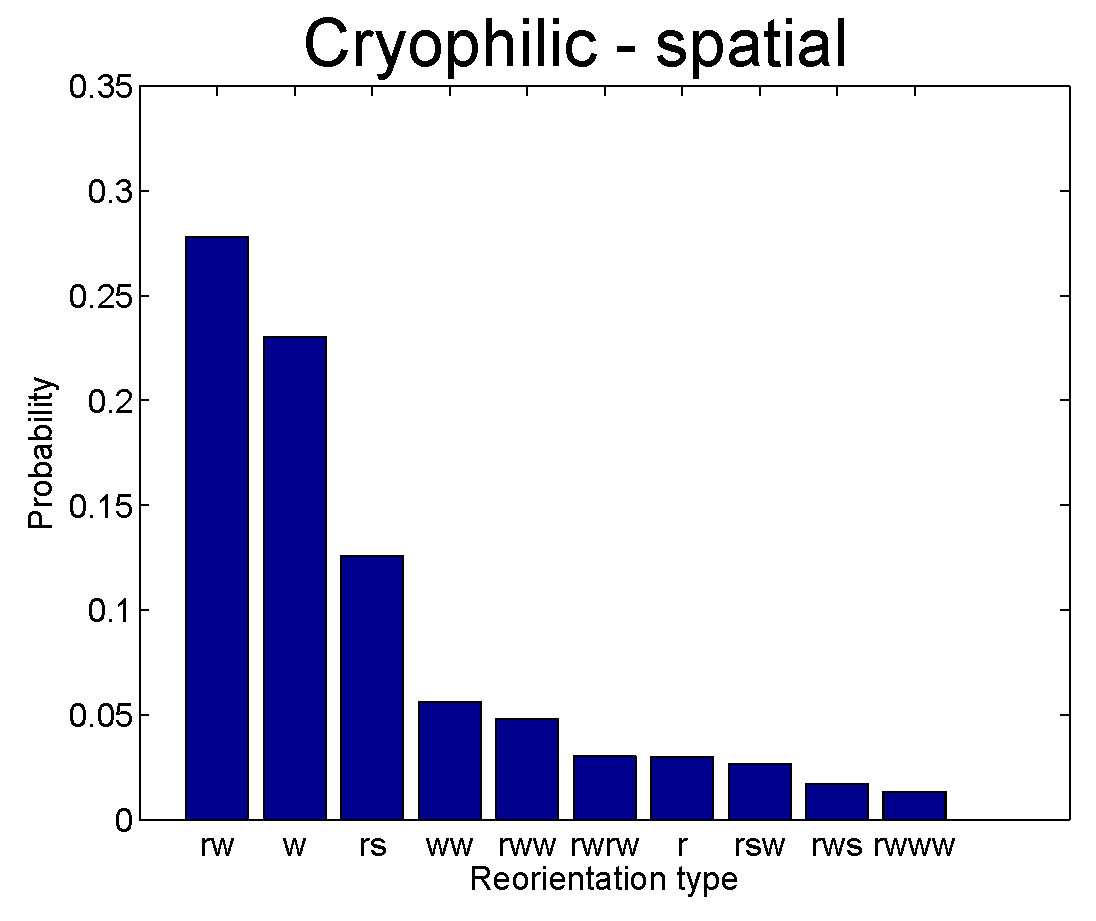
\includegraphics[width=6cm]{ReoTypeProb-cryospat.eps}
    (c)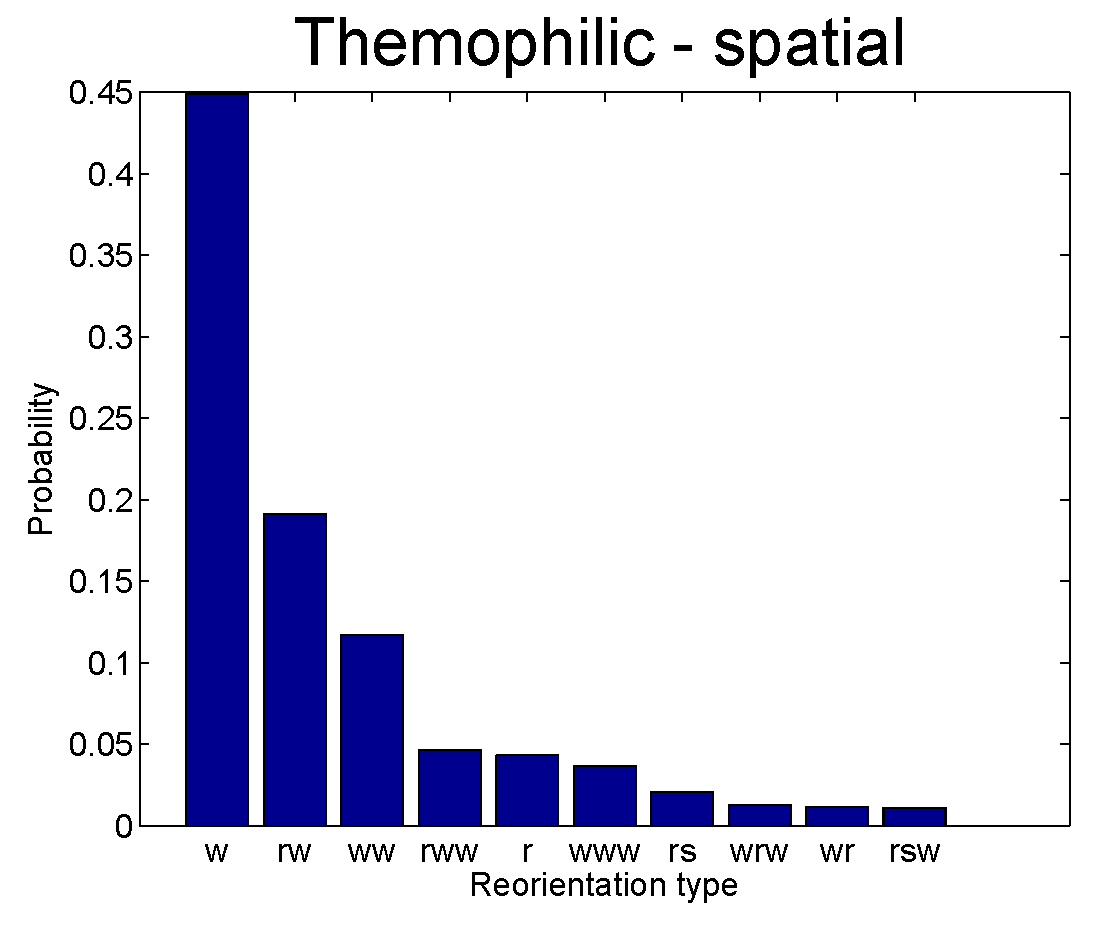
\includegraphics[width=6cm]{ReoTypeProb-thermospat.eps}\\[1cm]
    (d)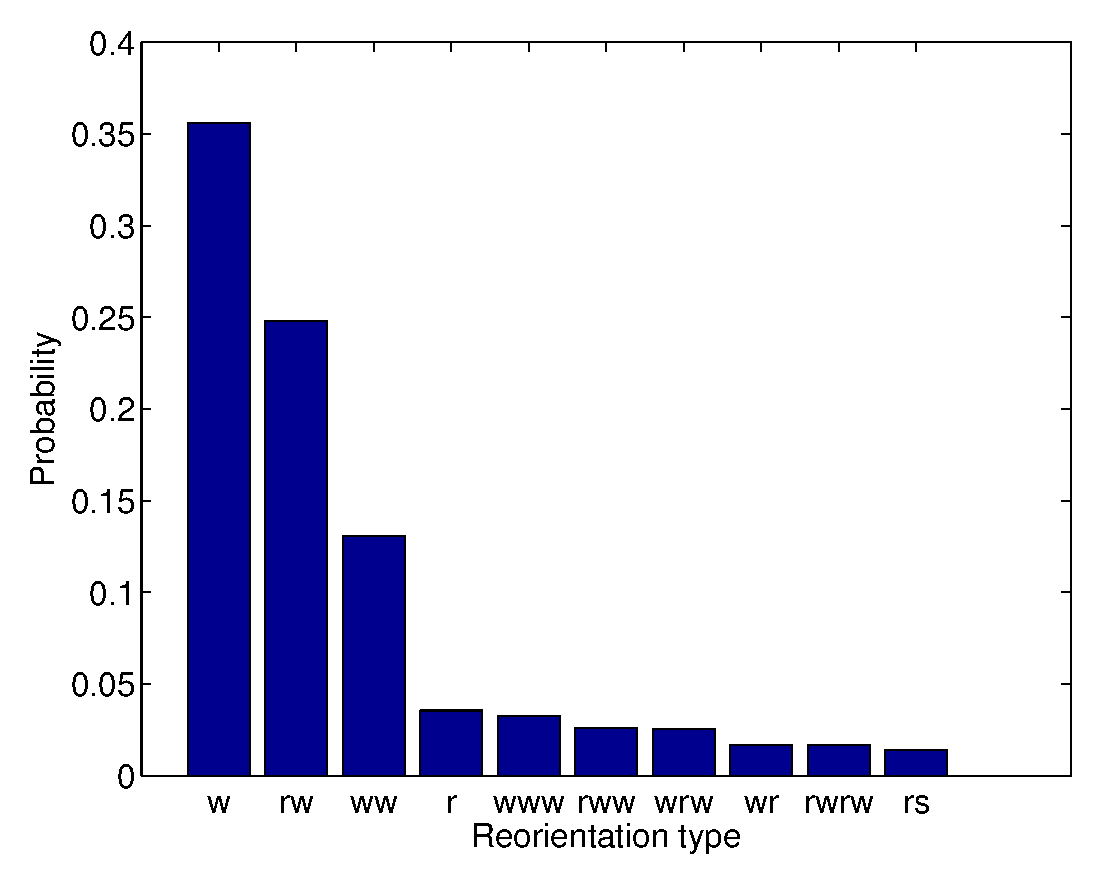
\includegraphics[width=6cm]{ReoTypeProb-lowsalt.eps}
    (e)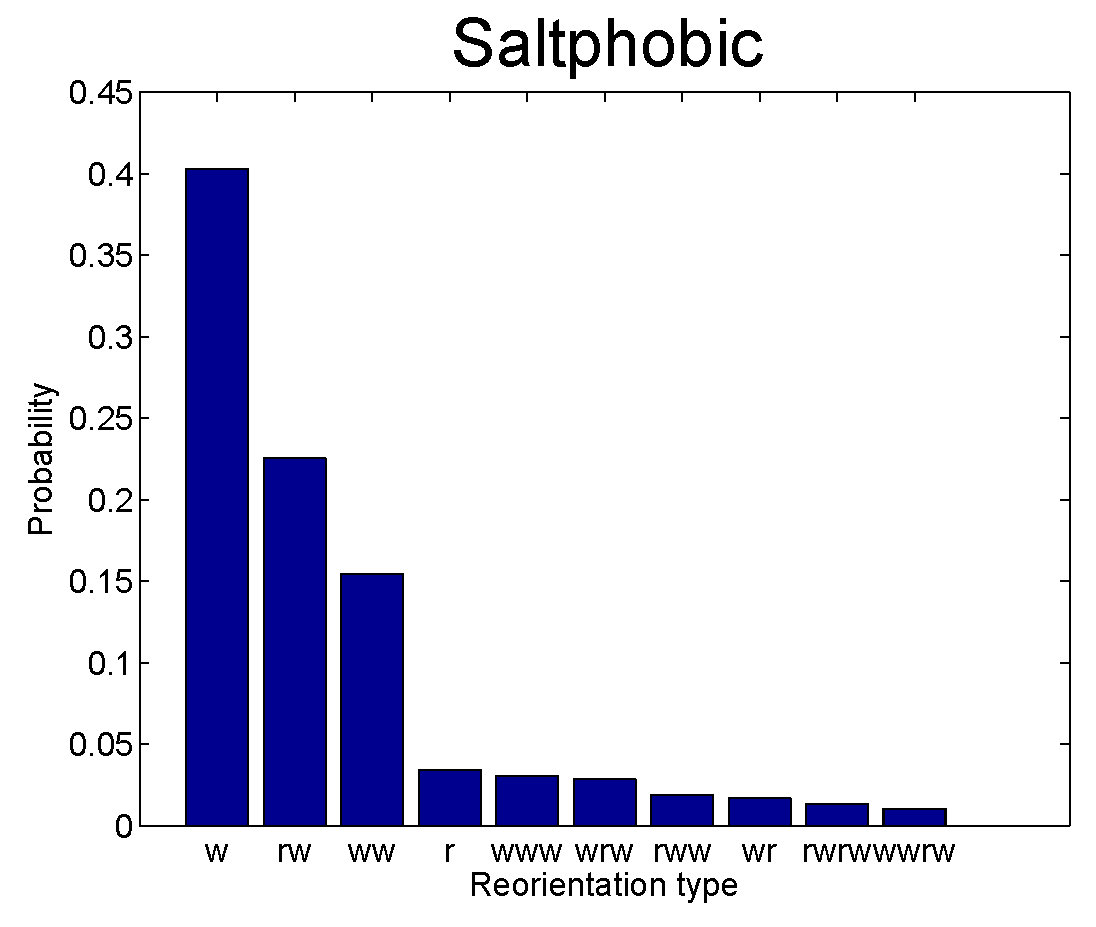
\includegraphics[width=6cm]{ReoTypeProb-highsalt.eps}
  \end{center}
  %\input{.TpX}
  \caption[Probabilities of different reorientation types.]{Probabilities of different reorientation types for (a) worms grown at $20\dC$ on no gradient at $20\dC$, (b) worms grown at $15\dC$ on spatial gradient from $18-23\dC$, (c)  worms grown at $25\dC$ on spatial gradient from $18-23\dC$, (d)  worms grown on $50\mM$ salt on spatial gradient from $0-50\mM$, (e)  worms grown on $50\mM$ salt on spatial gradient from $50-100\mM$.  Reorientation labels: w - Omega turn, r - reversal, s - unreversal. }\label{fig:typeprob}
\end{figure}


\begin{figure}
  \begin{center}
    (a)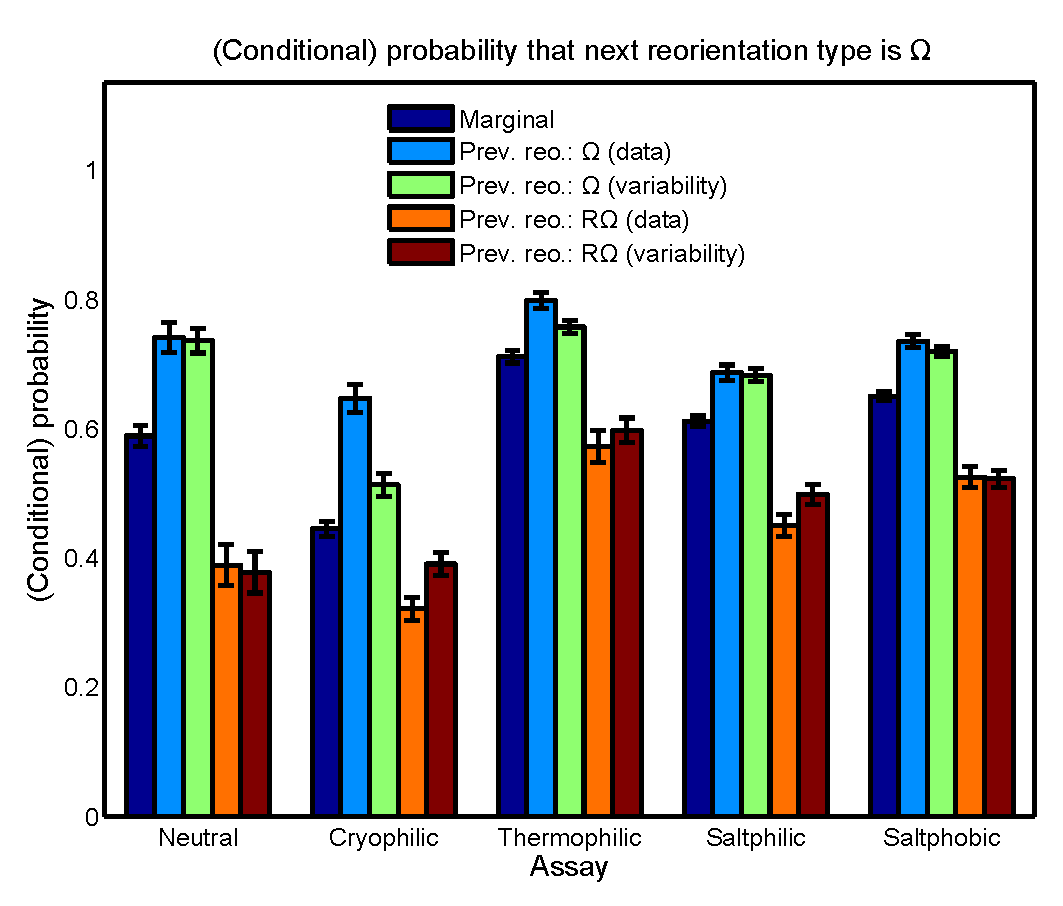
\includegraphics[width=7cm]{cond_type.eps}
    (b)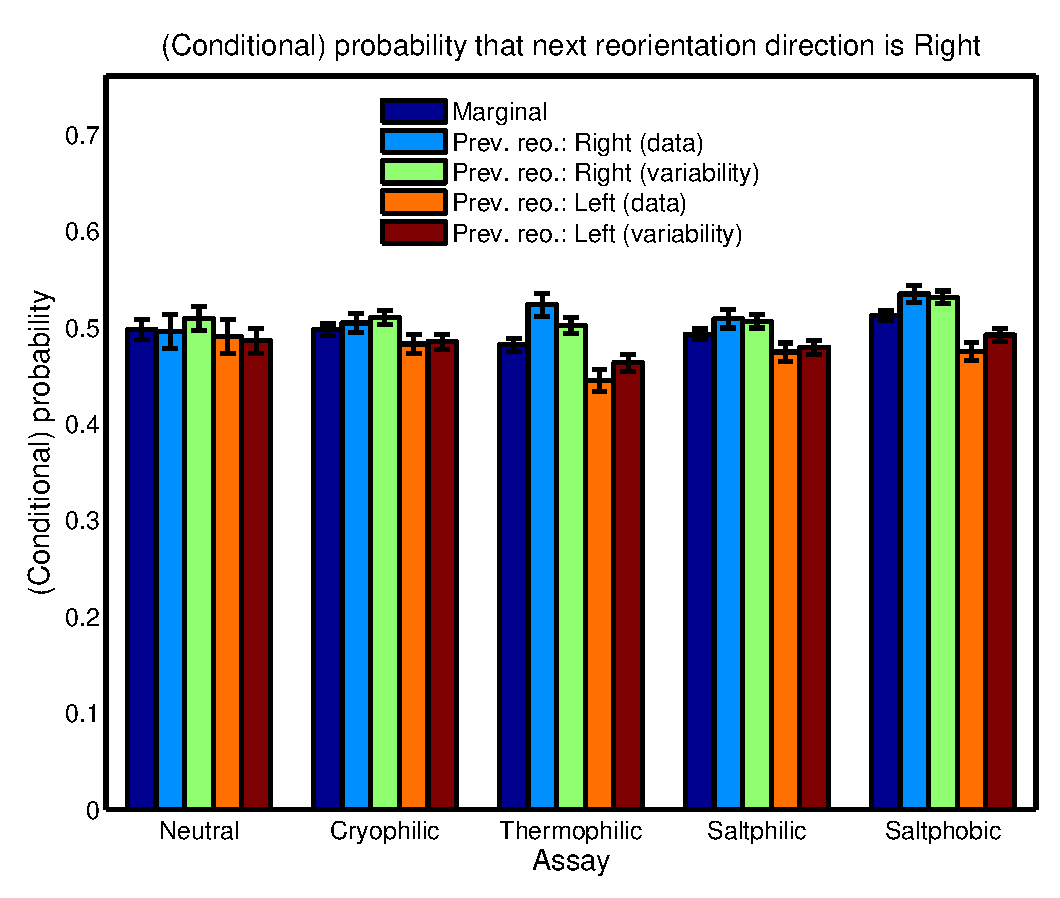
\includegraphics[width=7cm]{cond_dir.eps}\\[1cm]
    (c)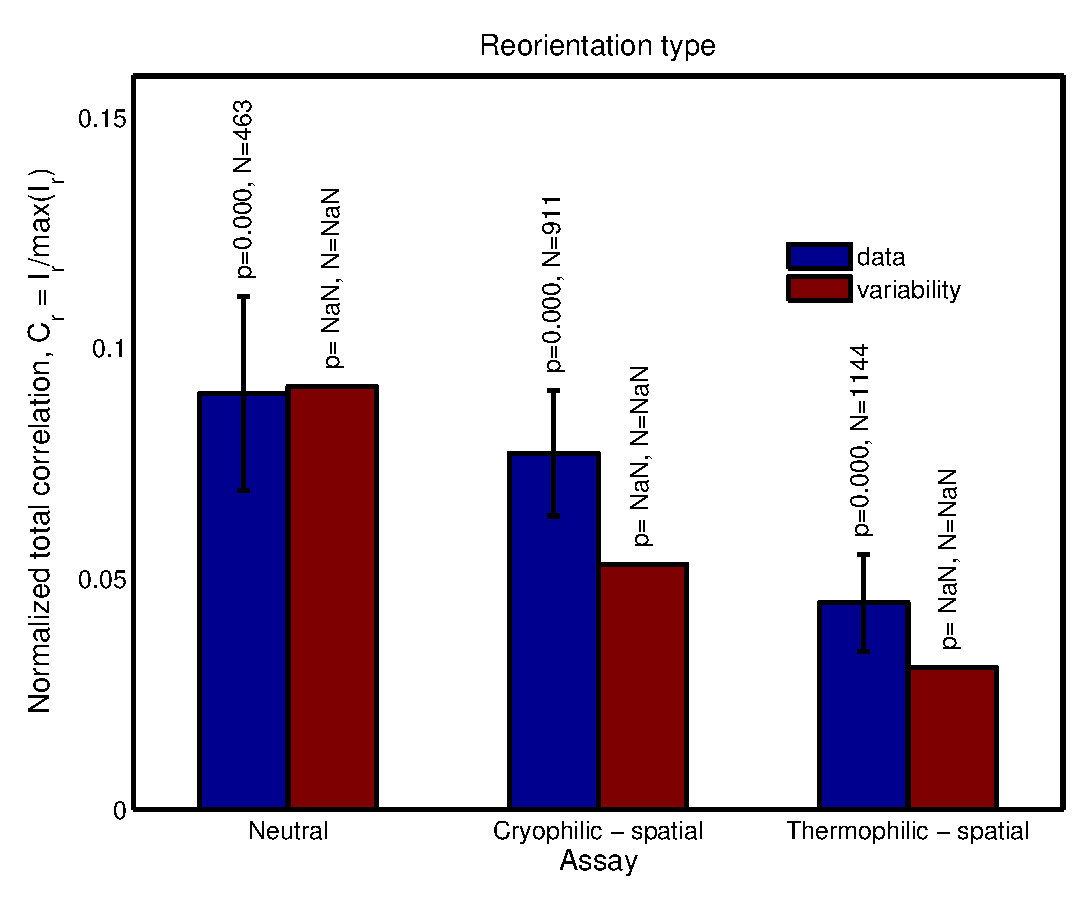
\includegraphics[width=7cm]{reotype_bin.eps}
    (d)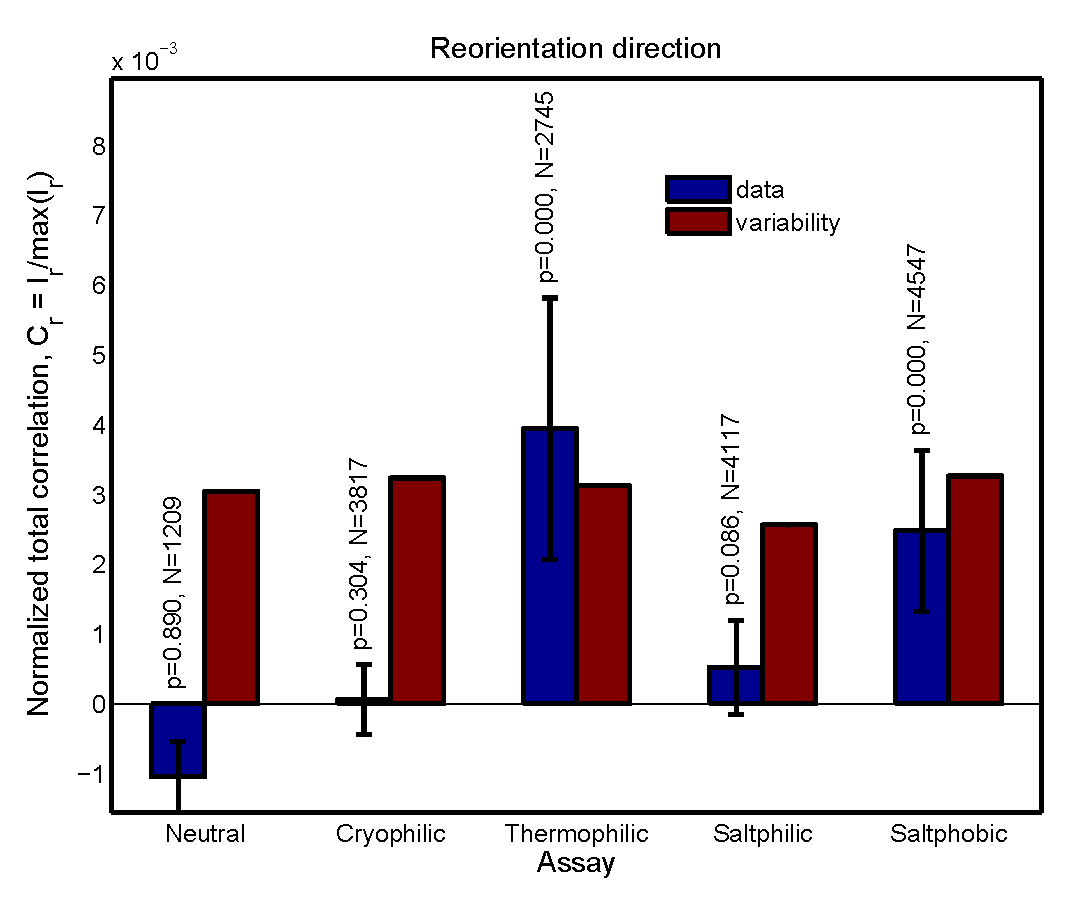
\includegraphics[width=7cm]{reoangle_bin.eps}
  \end{center}
  \caption[Conditional probabilities and mutual information (binary).]{Conditional probabilities and mutual information for worms grown at $20\dC$ on no gradient at $20\dC$,
  worms grown at $15\dC$ on spatial gradient from $18-23\dC$ over $22\cm$,
  worms grown at $25\dC$ on spatial gradient from $18-23\dC$ over $22\cm$,
  worms grown on $50\mM$ salt on spatial gradient from $0-50\mM$ over $22\cm$,
  worms grown on $50\mM$ salt on spatial gradient from $50-100\mM$ over $22\cm$.
  (a-b) Conditional probabilities for
  (a) reorientation types and
  (b) reorientation directions.
  Data refers to the actual measured values, variability refers to the predictions assuming that the only effect is due to animal-to animal variability as discussed in \sref{sec:variability}, with the variability measured as discussed in \sref{sec:variest}.
  (c-d) Normalised total correlation/mutual information in successive
  (c) reorientation types and
  (d) reorientation angles.
  Values have bias subtracted using the methods of appendix \ref{sec:stderr}. Error bars are one standard error, computed using the methods of appendix \ref{sec:stderr}.
  P-values for ``data'' are the probability that it is nonzero, they were computed using 1000 nonparametric bootstrap resamples under the null hypothesis that successive reorientations are independent, therefore the third decimal place is untrustworthy.
  $N$ is the number of $r$-tuples in the sample.
  P-values for ``variability'' are for the difference between it and ``data'', they were computed with a Z-test.} \label{fig:binaryresults}
\end{figure}


\begin{table}
  %
  \begin{center}
  (a) Reorientation type\\
  \begin{tabular}{|r|l|l|l|l|}
    \hline
    % after \\: \hline or \cline{col1-col2} \cline{col3-col4} ...
    \multirow{3}{*}{Assay} & \multicolumn{4}{|c|}{Comparison to} \\
    \cline{2-5}
      & \multicolumn{2}{|c|}{Marginal} & \multicolumn{2}{|c|}{Variability} \\
      \cline{2-5}
      & $P(\Omega|\Omega)$ & $P(\Omega|R\Omega)$ & $P(\Omega|\Omega)$ & $P(\Omega|R\Omega)$ \\
    \hline
    Neutral      & $1\ee{-8}$ & $2\ee{-8}$ & $0.9$ & $0.8$ \\
    Cryophilic   & $2\ee{-16}$ & $5\ee{-9}$ & $2\ee{-6}$ & $5\ee{-3}$ \\
    Thermophilic & $3\ee{-8}$ & $1\ee{-7}$ & $0.01$ & $0.4$ \\
    Saltphilic   & $1\ee{-7}$ & $4\ee{-17}$ & $0.8$ & $0.04$ \\
    Saltphobic   & $2\ee{-11}$ & $3\ee{-12}$ & $0.2$ & $0.9$ \\
    \hline
  \end{tabular}

  \vspace{1cm}

  (b) Reorientation direction\\
  \begin{tabular}{|r|l|l|l|l|}
    \hline
    % after \\: \hline or \cline{col1-col2} \cline{col3-col4} ...
    \multirow{3}{*}{Assay} & \multicolumn{4}{|c|}{Comparison to} \\
    \cline{2-5}
      & \multicolumn{2}{|c|}{Marginal} & \multicolumn{2}{|c|}{Variability} \\
      \cline{2-5}
      & $P(R|R)$ & $P(R|L)$ & $P(R|R)$ & $P(R|L)$ \\
    \hline
    Neutral      & $0.9$ & $0.7$ & $0.5$ & $0.9$ \\
    Cryophilic   & $0.6$ & $0.2$ & $0.6$ & $0.8$ \\
    Thermophilic & $2\ee{-3}$ & $5\ee{-3}$ & $0.1$ & $0.2$ \\
    Saltphilic   & $0.1$ & $0.09$ & $0.8$ & $0.7$ \\
    Saltphobic   & $0.03$ & $5\ee{-4}$ & $0.8$ & $0.1$ \\
    \hline
  \end{tabular}
  \end{center}
  %
  \caption[P-values for differences in conditional probabilities.]{P-values for differences in conditional probabilities for (a) reorientation type and (b) reorientation direction (data in \fref{fig:binaryresults}), computed with Z-tests.}\label{tab:condpval}
\end{table}


\subsection{The effect of reorientation type on reorientation direction}\label{sec:dirvstype}

\begin{figure}
\begin{center}
  (a)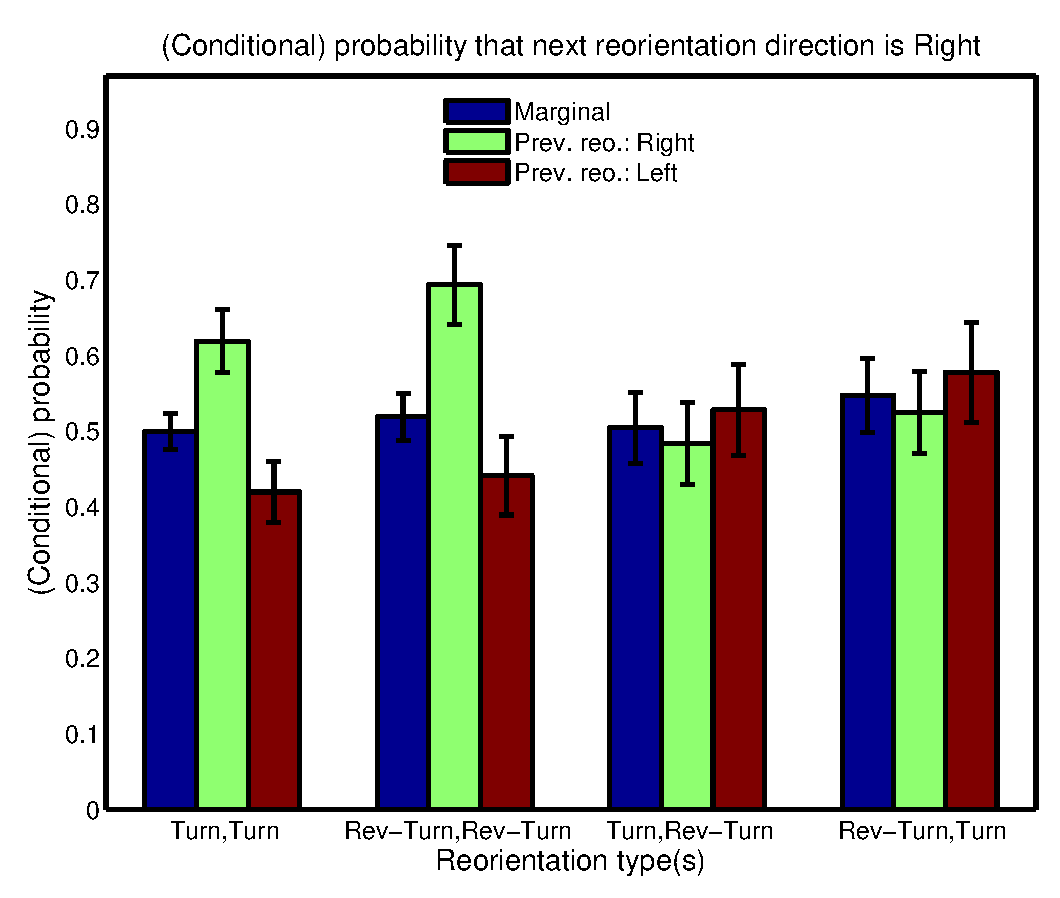
\includegraphics[width=7cm]{cond_dir_vs_type_(neutral).eps}\\
  (b)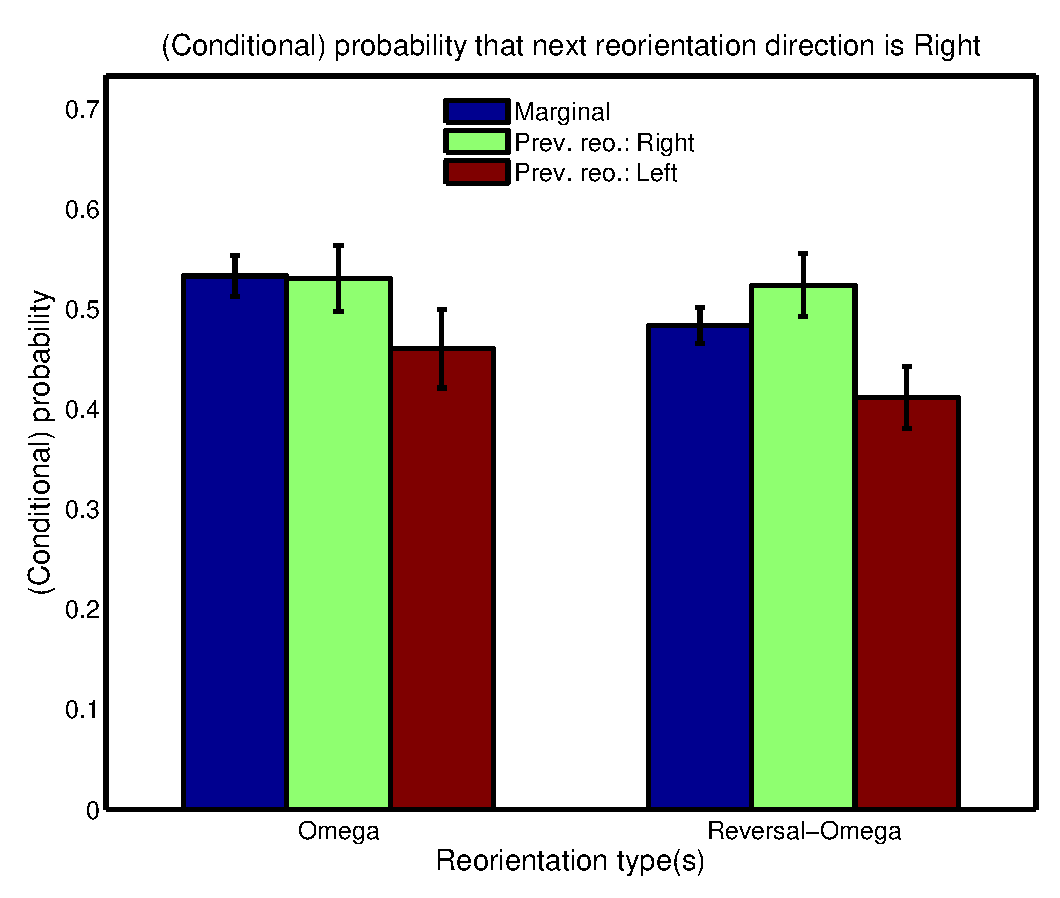
\includegraphics[width=7cm]{cond_dir_vs_type_(cryophilic).eps}
  (c)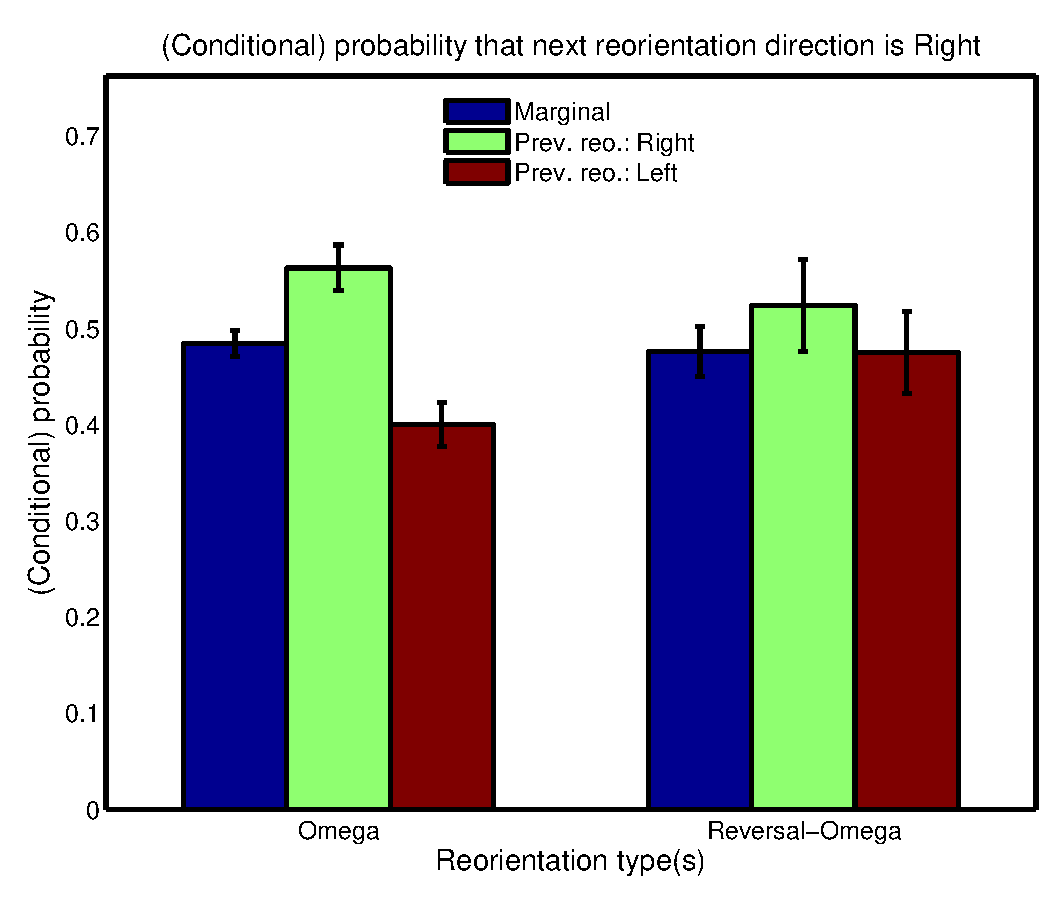
\includegraphics[width=7cm]{cond_dir_vs_type_(thermophilic).eps}\\
  (d)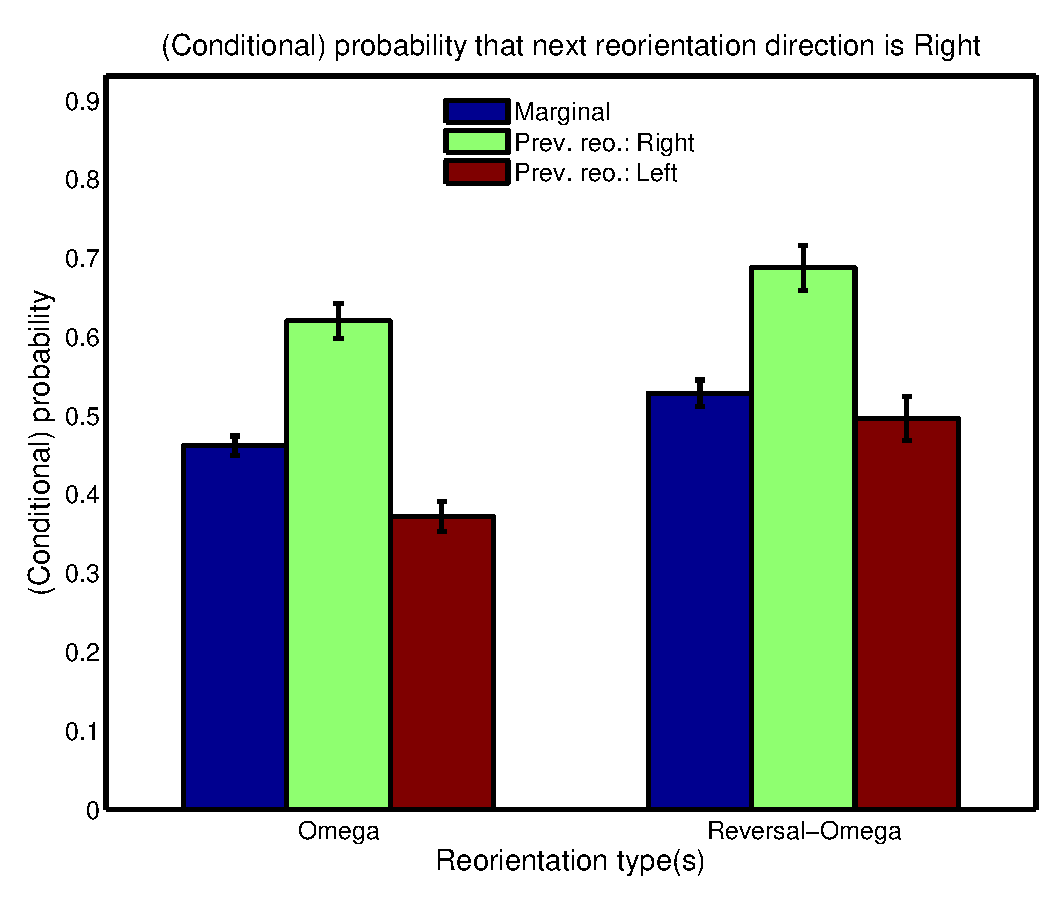
\includegraphics[width=7cm]{cond_dir_vs_type_(saltphilic).eps}
  (e)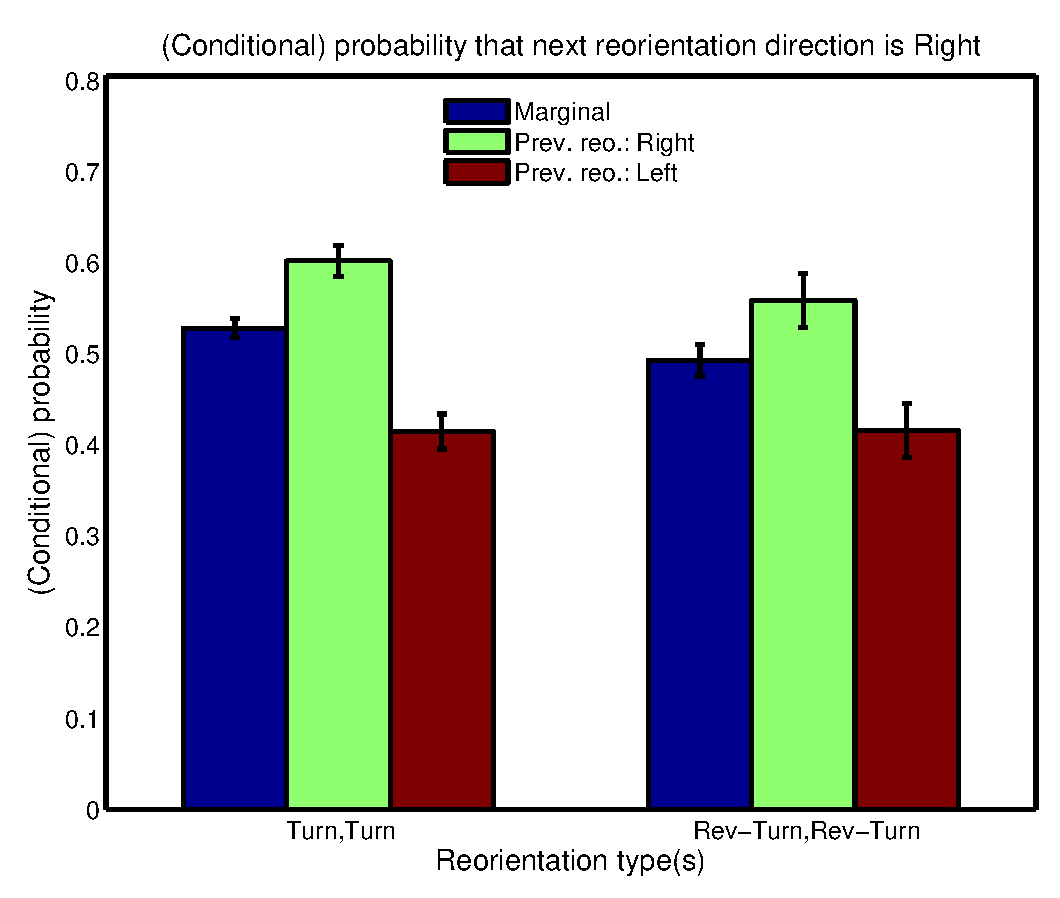
\includegraphics[width=7cm]{cond_dir_vs_type_(saltphobic).eps}
\end{center}
  %\input{.TpX}
  \caption[Conditional probabilities for reorientation direction restricted to certain reorientation types.]{Conditional probabilities for reorientation direction restricted to certain reorientation types for
  (a) worms grown at $20\dC$ on no gradient at $20\dC$,
  (b) worms grown at $15\dC$ on spatial gradient from $18-23\dC$ over $22\cm$,
  (c) worms grown at $25\dC$ on spatial gradient from $18-23\dC$ over $22\cm$,
  (d) worms grown on $50\mM$ salt on spatial gradient from $0-50\mM$ over $22\cm$,
  (e) worms grown on $50\mM$ salt on spatial gradient from $50-100\mM$ over $22\cm$.}\label{fig:dirvstype}
\end{figure}

\begin{table}
  %
  \begin{center}
  \begin{tabular}{|r|l|l|l|l|}
    \hline
    % after \\: \hline or \cline{col1-col2} \cline{col3-col4} ...
    \multirow{2}{*}{Assay} & \multicolumn{2}{|c|}{Omega} & \multicolumn{2}{|c|}{Reversal-Omega} \\
      \cline{2-5}
      & $P(R|R)$ & $P(R|L)$ & $P(R|R)$ & $P(R|L)$ \\
    \hline
    Neutral      & $0.01$ & $0.09$ & $0.004$ & $0.2$ \\
    Cryophilic   & $0.95$ & $0.1$ & $0.3$ & $0.05$ \\
    Thermophilic & $0.004$ & $0.002$ & $0.4$ & $0.99$ \\
    Saltphilic   & $6\ee{-10}$ & $8\ee{-5}$ & $0.8$ & $0.3$ \\
    Saltphobic   & $2\ee{-4}$ & $2\ee{-7}$ & $2\ee{-6}$ & $0.02$ \\
    \hline
  \end{tabular}
  \end{center}
  %
  \caption[P-values for differences in conditional probabilities for reorientation direction restricted to certain reorientation types]{P-values for difference between marginal and conditional probabilities for reorientation direction restricted to certain reorientation types (data in \fref{fig:dirvstype}), computed with Z-tests.}\label{tab:dirvstype}
\end{table}




\subsection{Continuous cases}\label{sec:ctsresults}

We computed the mutual information in successive reorientation angles (the total change in heading direction during the reorientation)  and run durations (the time between this reorientations and the previous one). As these are continuous variables, the data has to be binned. We will follow the approach of \cite{Slonim:2005} and place the bins on quantiles of the data, preserving the coordinate invariance of the mutual information. In both cases, we will use 5 bins.

%The results of this analysis are presented in \fref{fig:results}. The analysis was performed for an isotropic assay (where the temperature was uniform and constant), a spatial assay (where the temperature was constant in time but varied linearly in space from $18-23\dC$ over $9\cm$) and a temporal assay (where the temperature was constant in space but varied sinusoidally in time from $19.7-21\dC$ with a period of $10\mins$). For the temporal assay, the analysis was also performed restricted to periods of warming ($\diff{T}{t} > \ee{-4}\mbox{}\dC/\s[]$) and cooling ($\diff{T}{t} < -\ee{-4}\mbox{}\dC/\mathrm{s}$).

The results of this analysis are presented in \fref{fig:ctsresults}. The analysis was performed for isotropic assays (where the temperature was held uniform and constant at $20\dC$) and spatial assays (where the temperature was constant in time but varied linearly in space from $18-23\dC$ over $22\cm$). These were done with worms cultivated at $20\dC$ (neutral), $15\dC$ (cryophilic) ant $25\dC$ (thermophilic).

We looked at the cases $r=2$ (pairs of consecutive reorientations) and $r=3$ (triplets of consecutive reorientations). We also restricted attention to pairs of reorientations whose starts were separated by less than $30\s$ as well as pairs separated by more than $30\s$.

%Note that when we impose a restriction on the separation of reorientations, it is no longer true that the marginal distributions of the first and second run durations in a pair are identical. This was not dealt with properly, so the corresponding bars have been excluded in \fref{fig:results}. If run duration can affect reorientation type or angle, this same problem could exist in those cases. In \fref{fig:results2} we repeat the analysis using \eqref{eq:normmutinfgen} instead of \eqref{eq:normmutinf} for these cases only, in which case the uncertainty and bias can be calculated using the methods of \cite{Roulston1999} without modification.

Note that when we impose a restriction on the separation of reorientations, it is no longer true that the marginal distributions of the first and second run durations in a pair are identical. If run duration can affect reorientation type or angle, this same problem could exist in those cases. Therefore we performed the analysis using \eqref{eq:normmutinfgen} instead of \eqref{eq:normmutinf} for these cases only, in which case the uncertainty and bias can be calculated using the methods of \cite{Roulston1999} without modification.

%\begin{figure}
%  \begin{center}
%    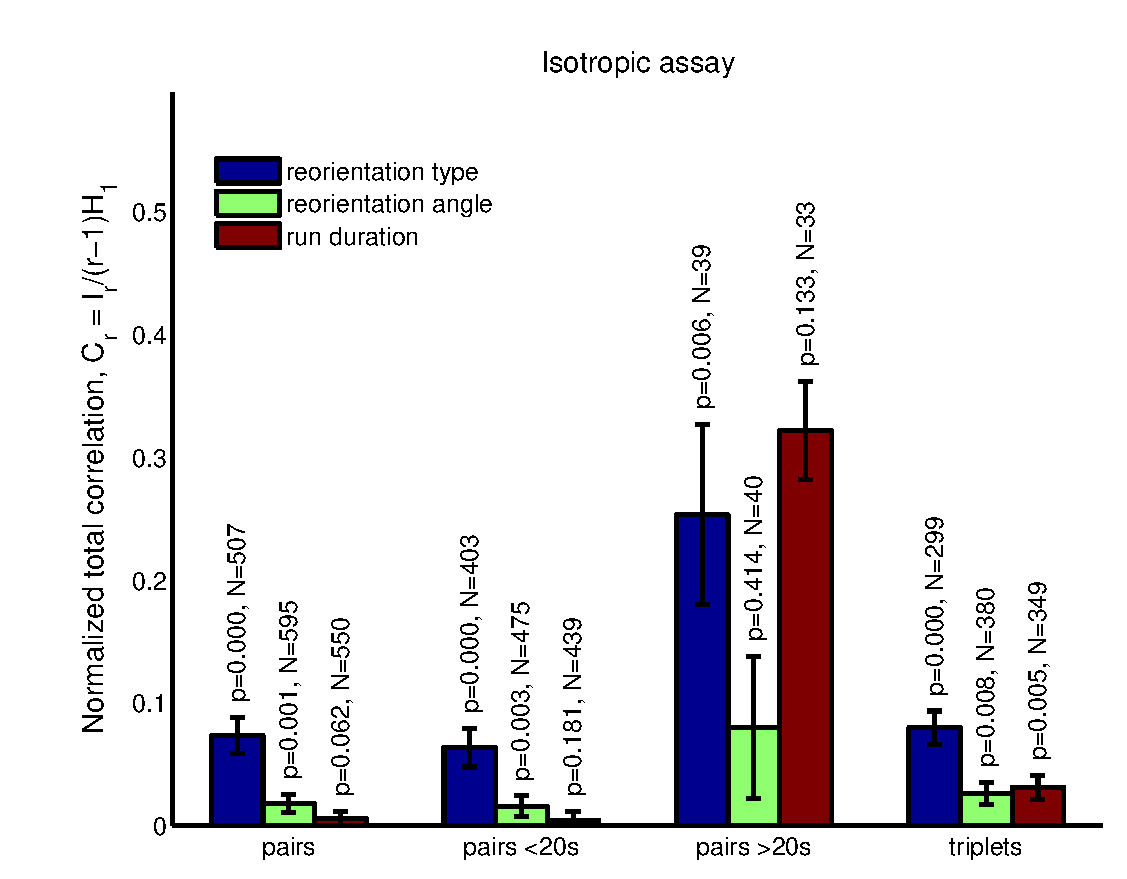
\includegraphics[width=8cm]{isotropic.eps}
%    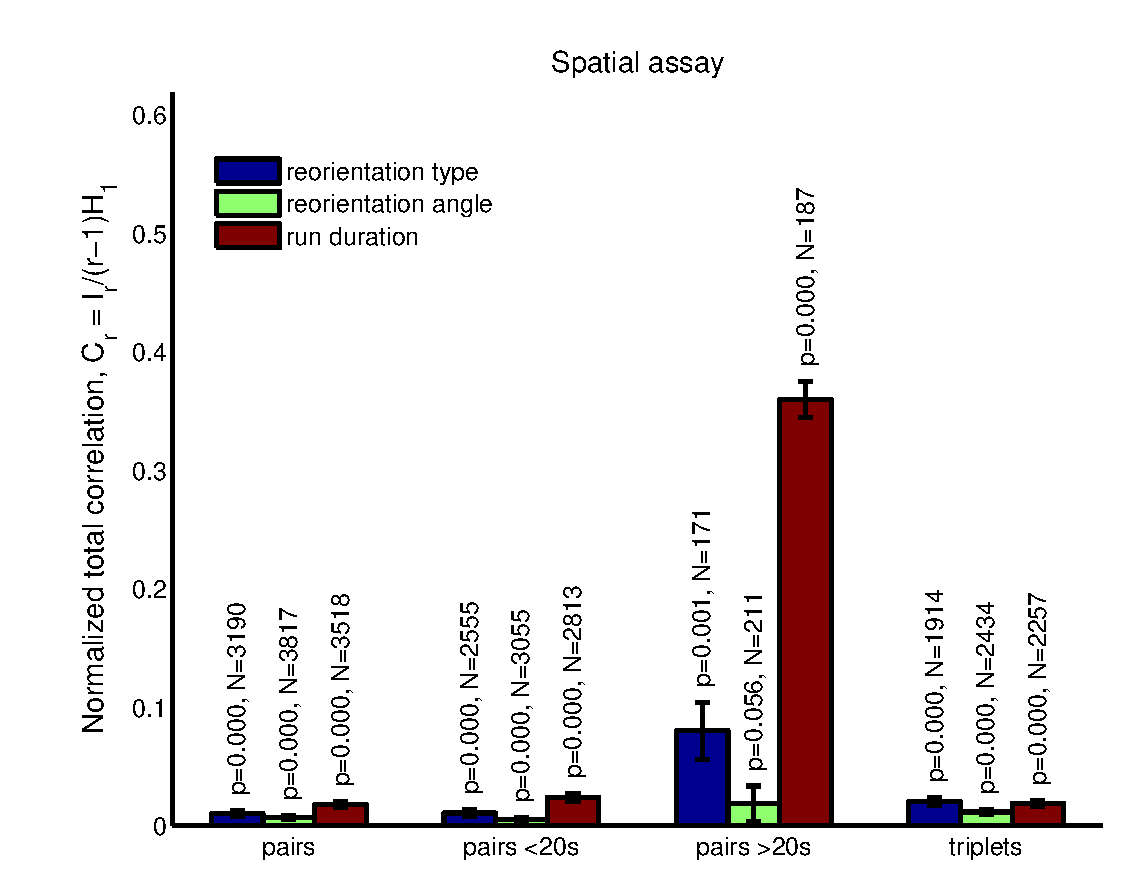
\includegraphics[width=8cm]{spatial.eps}\\
%    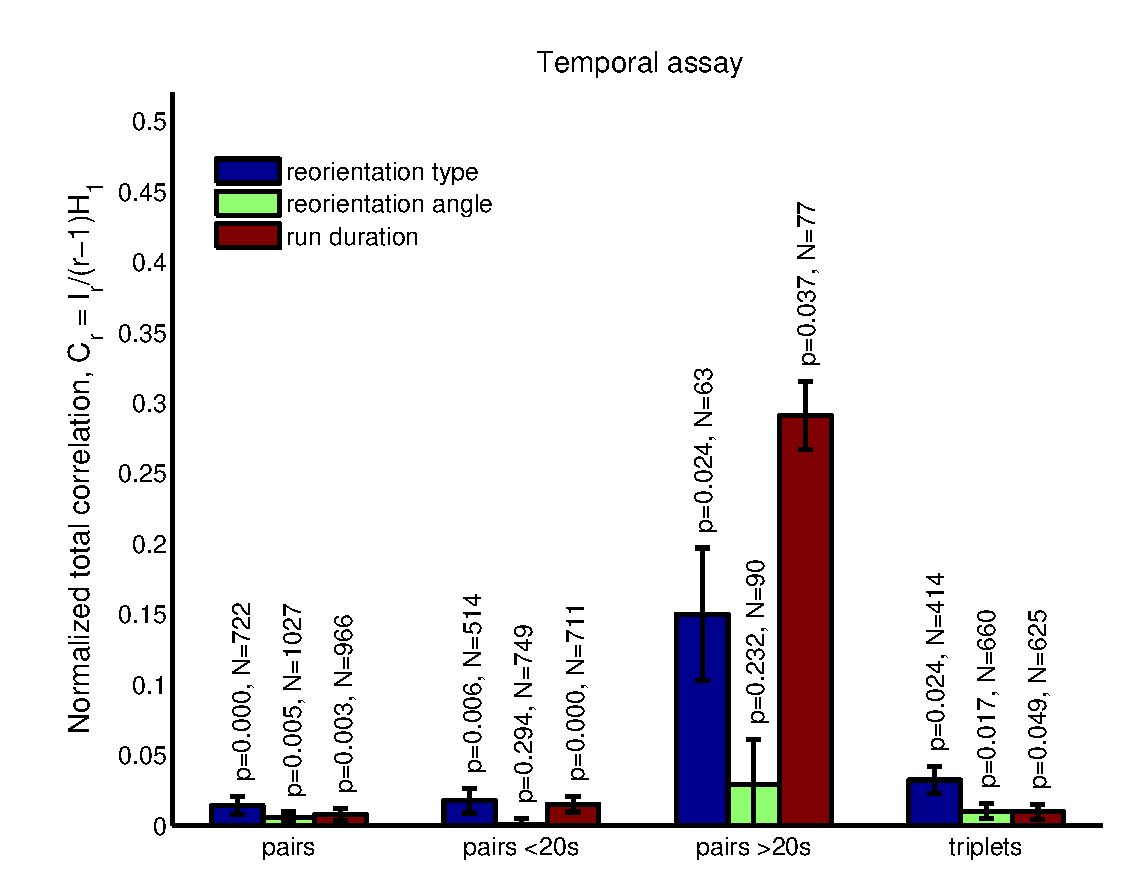
\includegraphics[width=8cm]{temporal.eps}
%    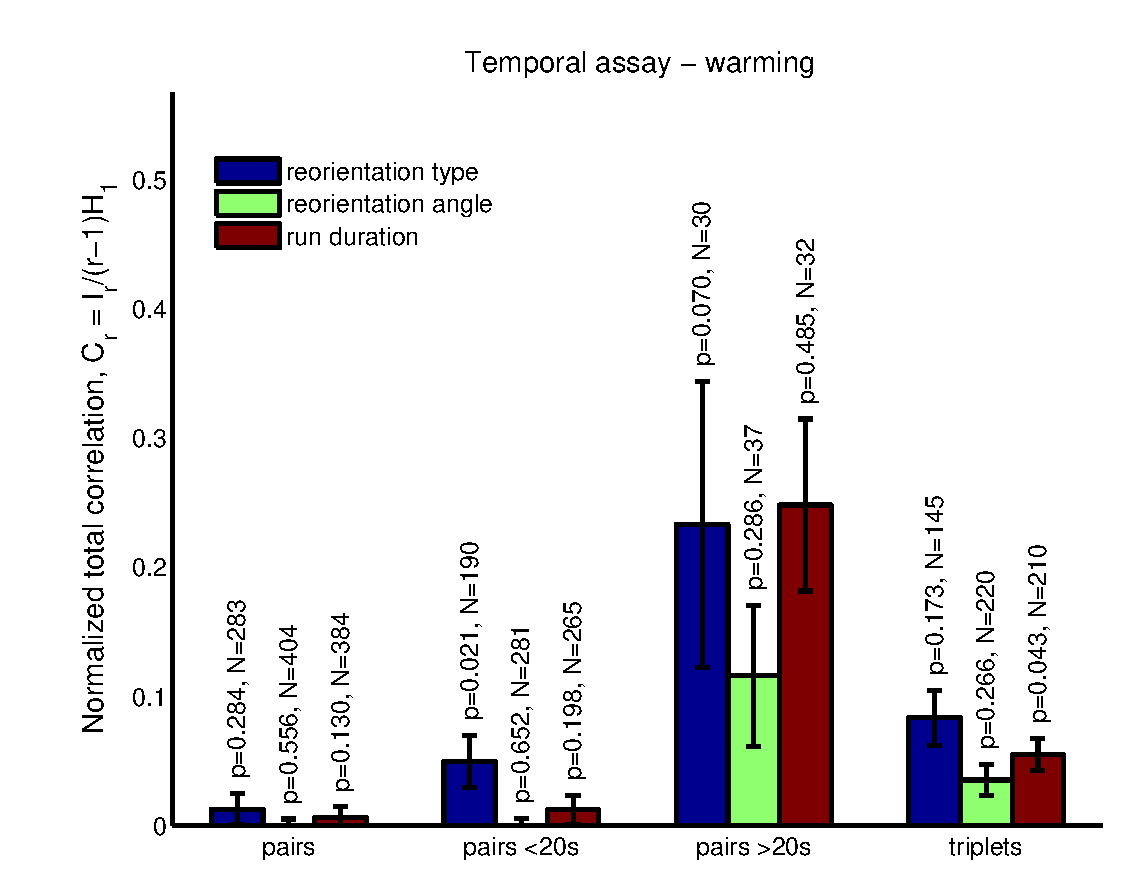
\includegraphics[width=8cm]{warming.eps}\\
%    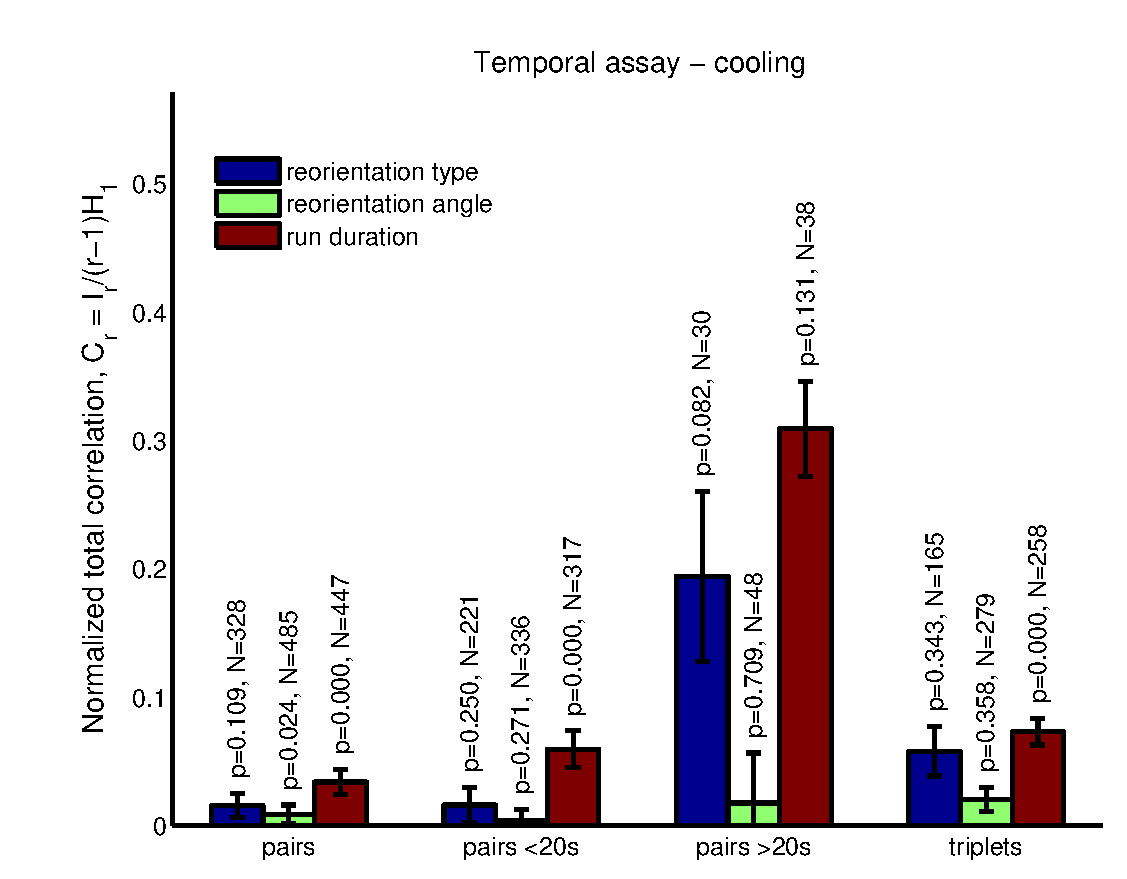
\includegraphics[width=8cm]{cooling.eps}
%  \end{center}
%  \caption{Normalised total correlation/mutual information for (a) isotropic assay, (b) spatial assay, (c) temporal assay, (d) temporal assay restricted to times when $\diff{T}{t} > 10^{-4}\mbox{}\dC/\mathrm{s}$, (e) temporal assay restricted to times when $\diff{T}{t} < -10^{-4}\mbox{}\dC/\mathrm{s}$. Values have bias subtracted using the methods of appendix \ref{sec:stderr}. Error bars are one standard error, computed using the methods of appendix \ref{sec:stderr}. P-values computed using 1000 nonparametric bootstrap resamples under the null hypothesis that successive reorientations are independent, therefore the third decimal place is untrustworthy. $N$ is the number of $r$-tuples in the sample.} \label{fig:results}
%\end{figure}

%\begin{figure}
%  \begin{center}
%    (a)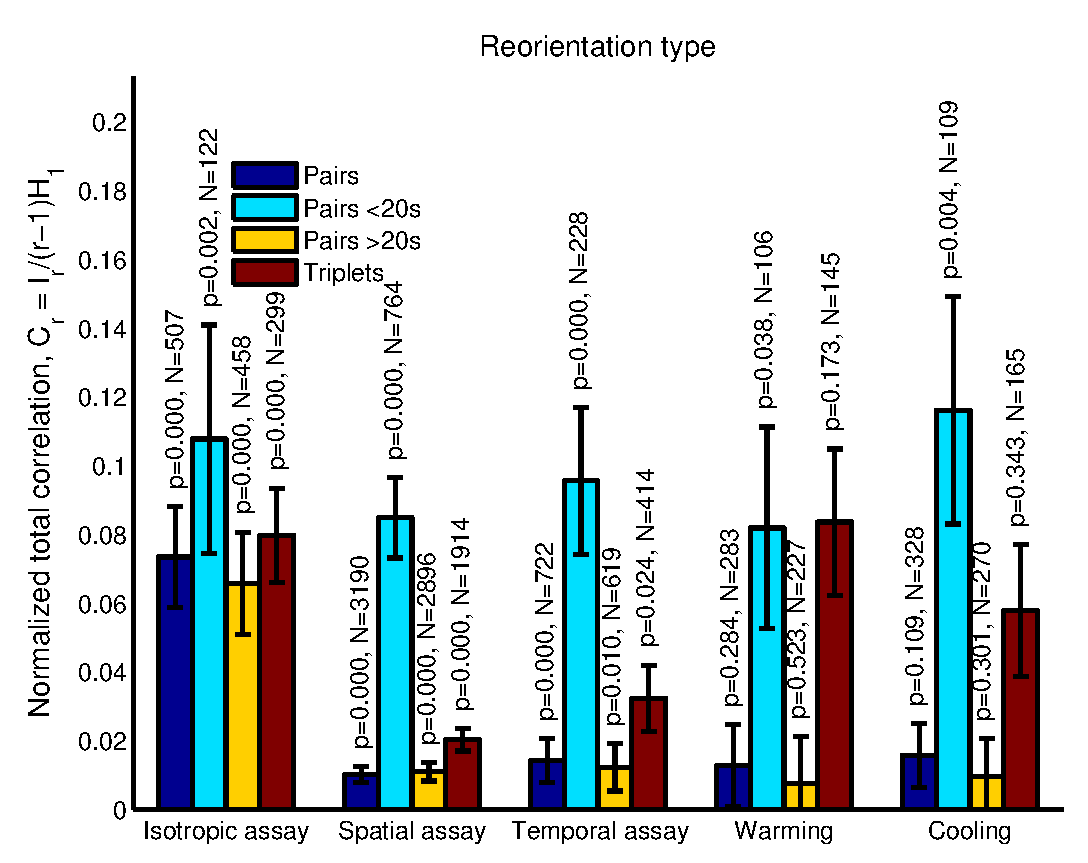
\includegraphics[width=7cm]{reotype.eps}
%    (b)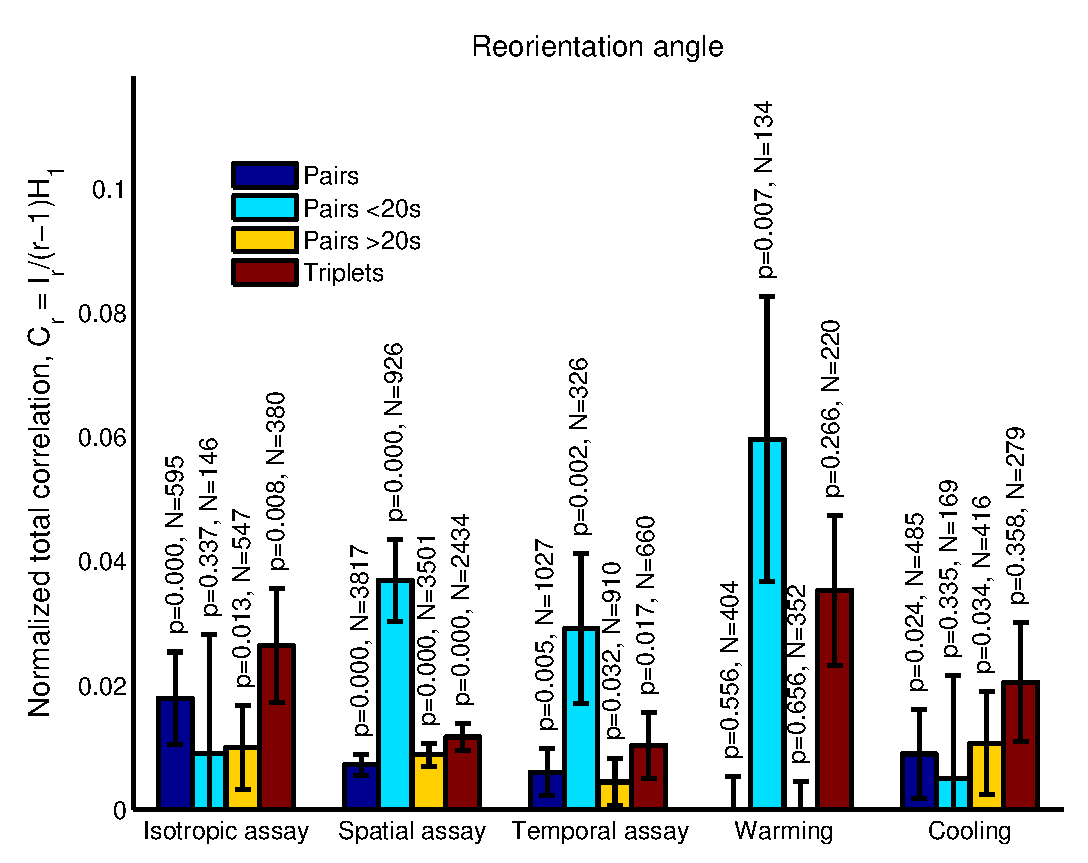
\includegraphics[width=7cm]{reoangle.eps}\\[1cm]
%    (c)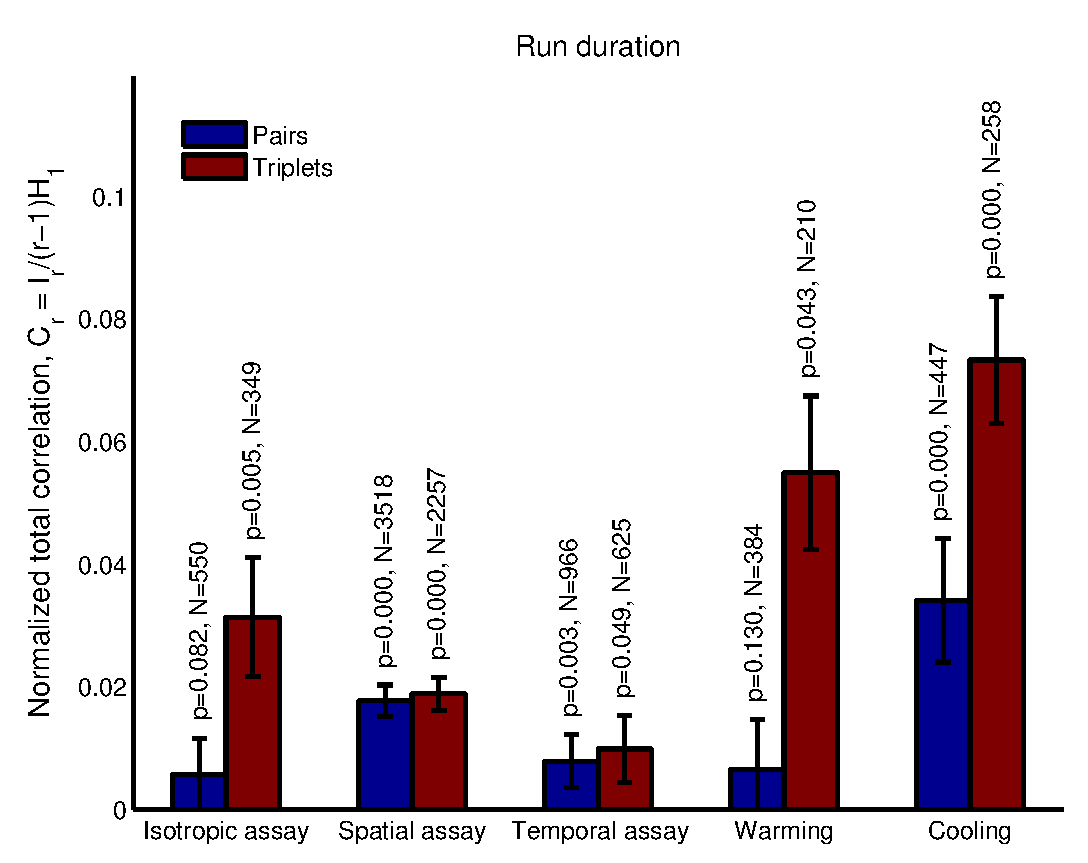
\includegraphics[width=7cm]{rundur.eps}
%  \end{center}
%  \caption{Normalised total correlation/mutual information in successive (a) reorientation types, (b) reorientation angles and (c) run durations for isotropic assay, spatial assay, temporal assay, temporal assay restricted to times when $\diff{T}{t} > 10^{-4}\mbox{}\dC/\mathrm{s}$ and temporal assay restricted to times when $\diff{T}{t} < -10^{-4}\mbox{}\dC/\mathrm{s}$. Values have bias subtracted using the methods of appendix \ref{sec:stderr}. Error bars are one standard error, computed using the methods of appendix \ref{sec:stderr}. P-values were computed using 1000 nonparametric bootstrap resamples under the null hypothesis that successive reorientations are independent, therefore the third decimal place is untrustworthy. $N$ is the number of $r$-tuples in the sample.} \label{fig:results}
%\end{figure}
%
%\begin{figure}
%  \begin{center}
%    (a)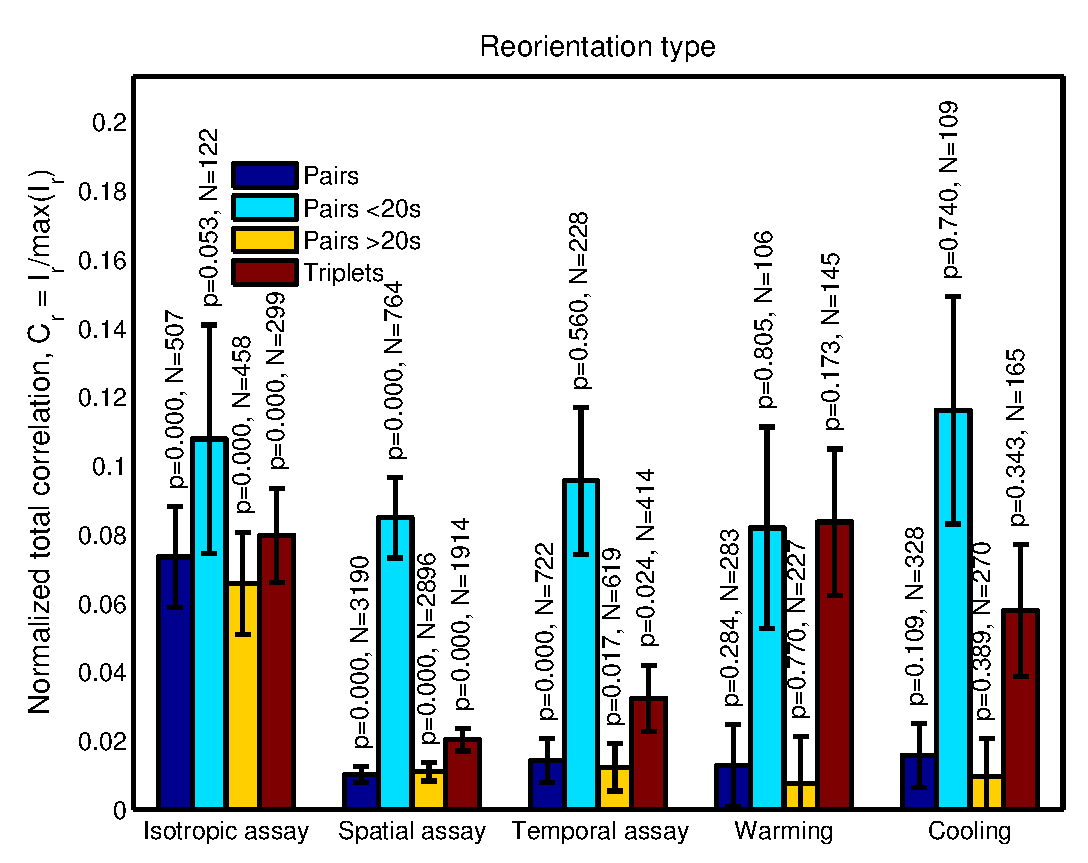
\includegraphics[width=7cm]{reotype2.eps}
%    (b)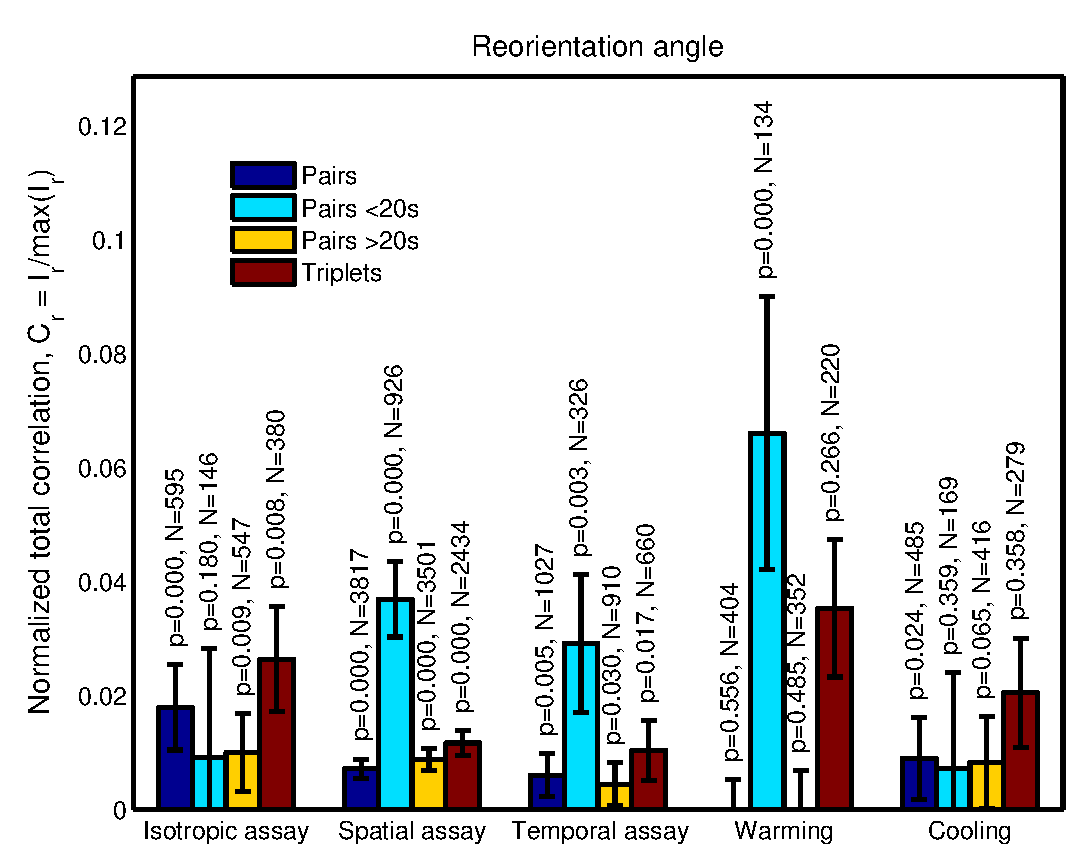
\includegraphics[width=7cm]{reoangle2.eps}\\[1cm]
%    (c)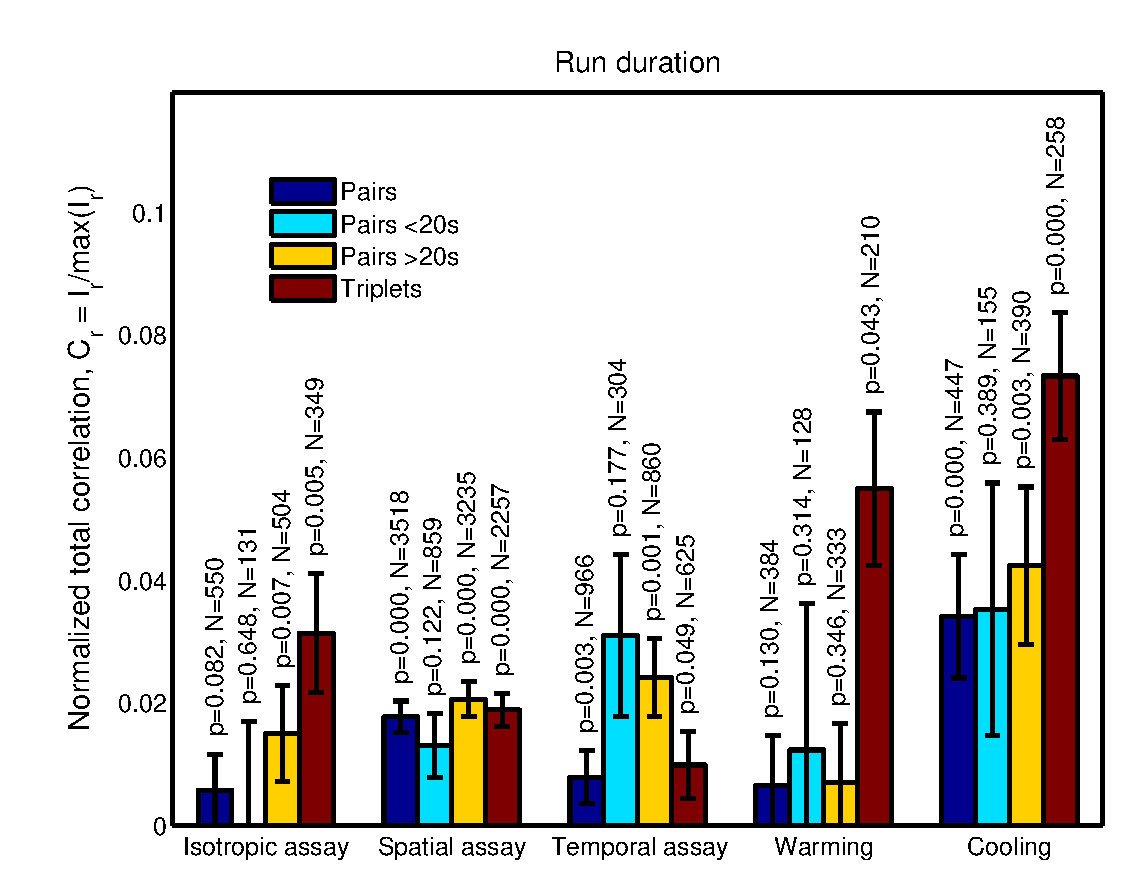
\includegraphics[width=7cm]{rundur2.eps}
%  \end{center}
%  \caption{Same as \fref{fig:results}, but we use \eqref{eq:normmutinfgen} instead of \eqref{eq:normmutinf} for the cases where we restrict attention to pairs of reorientations whose starts were separated by less than $20\s$ or pairs separated by more than $20\s$.} \label{fig:results2}
%\end{figure}

\begin{figure}
  \begin{center}
    (a)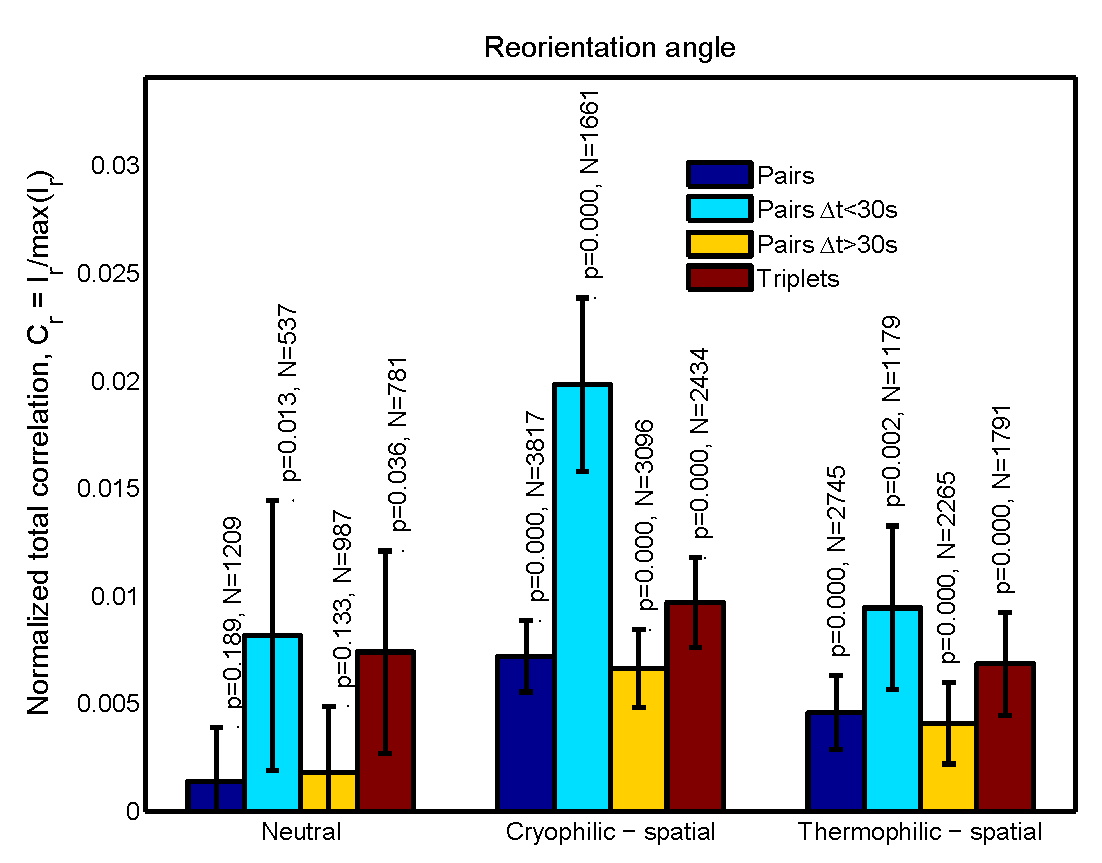
\includegraphics[width=7cm]{reoangle3.eps}
    (b)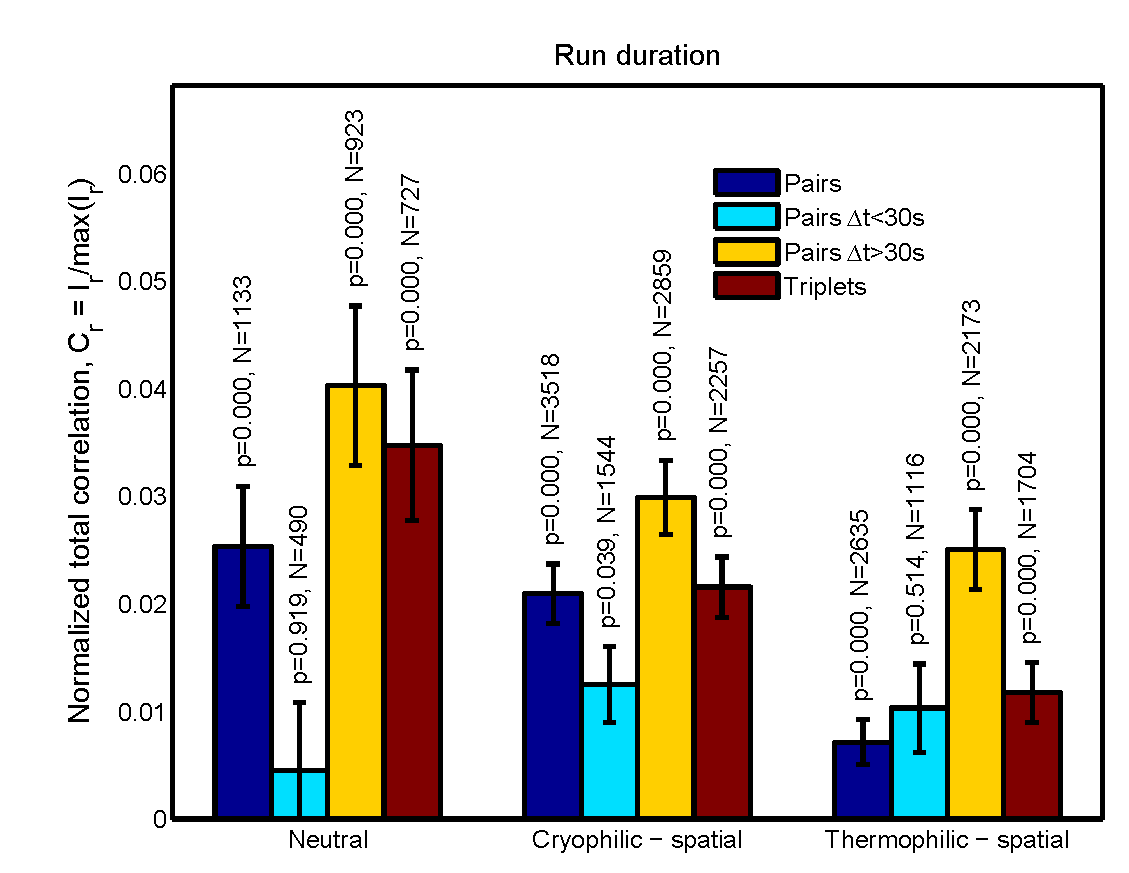
\includegraphics[width=7cm]{rundur3.eps}
  \end{center}
  \caption[Normalised total correlation/mutual information (continuous).]{Normalised total correlation/mutual information in successive (a) reorientation angles and (b) run durations for worms grown at $20\dC$ on no gradient at $20\dC$, worms grown at $15\dC$ on spatial gradient from $18-23\dC$ over $22\cm$ and worms grown at $25\dC$ on spatial gradient from $18-23\dC$ over $22\cm$. Values have bias subtracted using the methods of appendix \ref{sec:stderr}. Error bars are one standard error, computed using the methods of appendix \ref{sec:stderr}. P-values were computed using 1000 nonparametric bootstrap resamples under the null hypothesis that successive reorientations are independent, therefore the third decimal place is untrustworthy. $N$ is the number of $r$-tuples in the sample.} \label{fig:ctsresults}
\end{figure}




\appendix\section*{Appendices}

\section{Bias and standard error in entropy and mutual information}\label{sec:stderr}

We will follow the approach of \cite{Roulston1999}. Our situation is slightly different from that one. As all the $X_i$ have the same distribution, we will estimate $P(X)$ from the pooled data, rather that estimating the $P(X_i)$ separately. This means that our estimates may not satisfy the bounds, such as \eqref{eq:mutinfbounds}.

Let $p_{i_1\ldots i_r}$ denote the probability $P_r(X_1=x_{i_1},\ldots,X_r=x_{i_r})$ and $n_{i_1\ldots i_r}$ denote the number of corresponding r-tuples in the sample. We can estimate $p_{i_1\ldots i_r}$ with
%
\begin{equation}\label{eq:tupprob}
  q_{i_1\ldots i_r} = \frac{n_{i_1\ldots i_r}}{N},
  \qquad
  N = \sum_{j_1\ldots ji_r} n_{j_1\ldots j_r}.
\end{equation}
%
We can then estimate $p_{j}=P_1(X=x_{j})$ with
%
\begin{equation}\label{eq:singprob}
  q_j = \sum_{i_1\ldots i_r}\prn{ \frac{q_{i_1\ldots i_r}}{r} \sum_{a=1}^r \delta_{j,i_a}}.
\end{equation}
%

From now on, we will use $A$ to denote the estimate of $A(p)$ with $p$ replaced by $q$ and $\widehat{A}=A-\bias(A)$, where $A$ is one of $(H_1,H_r,I_r,C_r)$.

Our bias estimates are essentially the same as those of \cite{Roulston1999}, except that the number of samples for $H_1$ is $rN$ rather than $N$:
%
\begin{equation}\label{eq:biasH}
  B_1 = \bias(H_1) = -\frac{\#b_1}{2rN},
  \qquad
  B_r = \bias(H_r) = -\frac{\#b_r}{2N},
\end{equation}
%
where $\#b_r$ is the number of non-empty bins (\eg in \fref{fig:schematic}, $\#b_1=3$, $\#b_2=6$). The bias estimate for $I$ and $C$ follow in the usual way.

We can estimate the standard errors with
%
\begin{equation}\label{eq:stderr}
  \var(A) \approx \sum_{i_1\ldots i_r} \prn{\pdiff{A}{n_{i_1\ldots i_r}}}^2 \var(n_{i_1\ldots i_r}),
  \qquad
  \var(n_{i_1\ldots i_r}) \approx N q_{i_1\ldots i_r}(1-q_{i_1\ldots i_r}).
\end{equation}
%
where the first formula is valid provided each term is small(we'll see later that they are proportional to $1/N$) and the corrections to the last formula are lower order in $N$.

We find that
%
\begin{equation}\label{eq:dqbydn}
  \begin{aligned}
    \pdiff{q_{i_1\ldots i_r}}{n_{j_1\ldots j_r}} &= \frac{\prn{\prod_a \delta_{i_a,j_a}} - q_{i_1\ldots i_r}}{N}, &
    \qquad
    \pdiff{B_{r}}{n_{j_1\ldots j_r}} &= -\frac{B_r}{N},\\
    \pdiff{q_{i}}{n_{j_1\ldots j_r}} &= \frac{\frac{1}{r} \prn{\sum_a \delta_{i,j_a}} - q_{i}}{N}, &
    \pdiff{B_{1}}{n_{j_1\ldots j_r}} &= -\frac{B_1}{N},
   \end{aligned}
\end{equation}
%
which leads to
%
\begin{equation}\label{eq:dhbydn}
  \begin{aligned}
    \pdiff{H_r}{n_{j_1\ldots j_r}} &= -\frac{\log q_{j_1\ldots j_r} + H_r}{N}, &
    \qquad
    \pdiff{I_{r}}{n_{j_1\ldots j_r}} &= -\frac{\prn{\sum_a \log q_{j_a}}-\log q_{i_1\ldots i_r} + I_r}{N}, \\
    \pdiff{H_1}{n_{j_1\ldots j_r}} &= -\frac{\frac{1}{r} \prn{\sum_a \log q_{j_a}} + H_1}{N}, &
    \pdiff{C_{r}}{n_{j_1\ldots j_r}} &= \frac{\log q_{i_1\ldots i_r} H_1 - \frac{1}{r} \prn{\sum_a \log q_{j_a}} H_r}{(r-1)N(H_1)^2}.
   \end{aligned}
\end{equation}
%
All of these formulae are equally true if you put hats on every capital letter (except $N$).


\section{Bias and standard error in animal-to-animal variability}\label{sec:varibias}

In this appendix, we will concentrate on reorientation types. The generalisation to reorientation directions is trivial. Our approach is the same as that of \cite{Roulston1999}.

We have:
%
\begin{equation}\label{eq:estdist}
  P(\hat{p}_i|\hat{n}_i) \sim \frac{\mathrm{Binom}(\hat{n}_i,p_i)}{\hat{n}_i},
  \qquad
  P(\hat{n}_i) \sim \mathrm{Poisson}(r_it),
\end{equation}
%
where $r_i$ is the reorientation rate of animal $i$ and $t$ is the duration of the tracks. We also define
%
\begin{equation}\label{eq:biasnot}
  n_i = r_it, \qquad
  N_0 = \sum_i n_i, \qquad
  \epsilon_i = \frac{\hat{n}_i}{n_i}-1, \qquad
  q_i = \frac{r_i}{\sum_j r_j} = \frac{n_i}{N_0}.
\end{equation}
%

Expanding in $\epsilon_i$ leads to
%
\begin{equation}\label{eq:expandeps}
  \begin{aligned}
    \hat{q}_i &= q_i\brk{ 1 + \prn{\epsilon_i-\sum_jq_j\epsilon_j} -  \prn{\epsilon_i-\sum_jq_j\epsilon_j} \prn{\sum_kq_k\epsilon_k} } +\CO\prn{\epsilon_i^3}, \\
    \hat{q}_i\hat{q}_j &= q_iq_j\brk{ 1 + \prn{\epsilon_i+\epsilon_j-2\sum_kq_k\epsilon_k} +  \prn{\epsilon_i\epsilon_j-(\sum_kq_k\epsilon_k)^2} }  +\CO\prn{\epsilon_i^3}, \\
    \frac{1}{N} &= \frac{1}{N_0} \brk{ 1 - \prn{\sum_kq_k\epsilon_k} +  \prn{\sum_kq_k\epsilon_k}^2 } +\CO\prn{\epsilon_i^3}.
  \end{aligned}
\end{equation}
%
Using the Poisson distribution, one can show that
%
\begin{equation}\label{eq:expeps}
    \E\brk{\epsilon_i} = 0, \qquad
    \E\brk{\epsilon_i^2} = \frac{1}{n_i}, \qquad
    \E\brk{\epsilon_i^{k+3}} = \CO\prn{\frac{1}{n_i^2}} \quad k\geq0,
\end{equation}
%
and therefore
%
\begin{equation}\label{eq:expandepsex}
  \begin{aligned}
    \E\brk{\hat{q}_i} &= q_i + \CO\prn{\frac{1}{n_i^2}}, \\
    \E\brk{\hat{q}_i\hat{q}_j} &= q_iq_j\brk{ 1 + \frac{\delta_{ij}}{n_i} -  \frac{1}{N_0}}  + \CO\prn{\frac{1}{n_i^2}}, \\
    \E\brk{\frac{1}{N}} &= \frac{1}{N_0} \brk{ 1  +  \frac{1}{N_0} } + \CO\prn{\frac{1}{n_i^2}}.
  \end{aligned}
\end{equation}
%

Using the Binomial distribution, one can show that
%
\begin{equation}\label{eq:expi}
  \E\brk{\hat{p}_i|\hat{n}_i} = p_i, \qquad
  \E\brk{\hat{p}_i^2|\hat{n}_i} = p_i^2 + \frac{p_i(1-p_i)}{n_i}.
\end{equation}
%

The obvious estimator for $\bar{p}$ works just fine:
%
\begin{equation}\label{eq:pbarest}
  \E\brk{\sum_i\hat{q}_i\hat{p}_i\middle|\hat{n}_i} = \sum_i \hat{q}_ip_i,
  \qquad
  \E\brk{\sum_i\hat{q}_ip_i} + \CO\prn{\frac{1}{n_i^2}} = \sum_iq_ip_i = \bar{p} + \CO\prn{\frac{1}{n_i^2}}.
\end{equation}
%

However, the obvious estimator for $\sigma_p^2$ fails at the first hurdle:
%
\begin{equation}\label{eq:sigest1}
  \E\brk{\sum_i\hat{q}_i(\hat{p}_i-\hat{\bar{p}})^2\middle|\hat{n}_i} = \sum_i \hat{q}_i p_i^2 - \prn{\sum_i \hat{q}_ip_i}^2 + \sum_i \frac{\hat{q}_i (1-\hat{q}_i)p_i(1-p_i)}{\hat{n}_i}.
\end{equation}
%
We can correct this,
%
\begin{equation}\label{eq:sigest2}
  \E\brk{\sum_i\hat{q}_i(\hat{p}_i-\hat{\bar{p}})^2 - \sum_i \frac{\hat{q}_i (1-\hat{q}_i)\hat{p}_i(1-\hat{p}_i)}{\hat{n}_i-1} \middle|\hat{n}_i} = \sum_i \hat{q}_i p_i^2 - \prn{\sum_i \hat{q}_ip_i}^2 ,
\end{equation}
%
but it fails at the next hurdle:
%
\begin{equation}\label{eq:sigest3}
  \E\brk{\sum_i \hat{q}_i p_i^2 - \prn{\sum_i \hat{q}_ip_i}^2 } = \frac{N_0-1}{N_0}\prn{\sum_i q_i p_i^2 - \prn{\sum_i q_ip_i}^2} + \CO\prn{\frac{1}{n_i^2}}.
\end{equation}
%
Luckily, this can be corrected:
%
\begin{equation}\label{eq:sigest4}
\begin{aligned}
  \E\brk{\frac{N_0+1}{N_0}\prn{\sum_i\hat{q}_i(\hat{p}_i-\hat{\bar{p}})^2 - \sum_i \frac{\hat{q}_i (1-\hat{q}_i)\hat{p}_i(1-\hat{p}_i)}{\hat{n}_i-1} } \middle|\hat{n}_i} &= \frac{N_0+1}{N_0}\prn{\sum_i \hat{q}_i p_i^2 - \prn{\sum_i \hat{q}_ip_i}^2} ,\\
  \E\brk{\frac{N_0+1}{N_0}\prn{\sum_i \hat{q}_i p_i^2 - \prn{\sum_i \hat{q}_ip_i}^2} } &= \sum_i q_i p_i^2 - \prn{\sum_i q_ip_i}^2 + \CO\prn{\frac{1}{n_i^2}} \\&= \sigma_p^2 + \CO\prn{\frac{1}{n_i^2}}.
\end{aligned}
\end{equation}
%

To estimate the variances, we use the approach
%
\begin{equation}\label{eq:estvarest}
  \var(\hat{A}) \approx \sum_i\prn{ \pdiffc{\hat{A}}{\Omega_i}^2 \var(\Omega_i) + \pdiffc{\hat{A}}{R_i}^2 \var(R_i) } = \sum_i\prn{ \pdiffc{\hat{A}}{\Omega_i}^2 \Omega_i + \pdiffc{\hat{A}}{R_i}^2 R_i }.
\end{equation}
%
This relatively simple for $\hat{\bar{p}}$:
%
\begin{equation}\label{eq:varpbar}
  \begin{aligned}
    \hat{\bar{p}} &= \sum_i \hat{q}_i \hat{p}_i = \sum_i \frac{\sum_i\Omega_i}{\sum_i(\Omega_i+R_i)}, \\
    \pdiff{\hat{\bar{p}}}{\Omega_i}  &= \frac{\sum_iR_i}{\prn{\sum_i(\Omega_i+R_i)}^2},\\
    \pdiff{\hat{\bar{p}}}{R_i}  &= -\frac{\sum_i\Omega_i}{\prn{\sum_i(\Omega_i+R_i)}^2},\\
    \var(\hat{\bar{p}}) &\approx \frac{\prn{\sum_i\Omega_i}\prn{\sum_iR_i}}{\prn{\sum_i(\Omega_i+R_i)}^3} = \frac{\hat{\bar{p}}(1-\hat{\bar{p}})}{N}.
  \end{aligned}
\end{equation}
%
but it is much more complicated for $\hat{\sigma}_p^2$:
%
\begin{equation}\label{eq:varsigmap}
  \begin{aligned}
    \pdiff{\sigma_p^2}{\Omega_i} =& -\frac{\hat{\sigma}_p^2}{N(N+1)} + \frac{N+1}{N} \prn{\frac{\hat{q}_i (1-\hat{q}_i) \hat{p}_i (1-\hat{p}_i)} {(\hat{n}_i-1)^2}}
    \\ &+
    \frac{N+1}{N^2} \prn{ \hat{p}_i^2 - (\sum_j \hat{q}_j\hat{p}_j^2) - 2 \hat{p}_i\hat{\bar{p}} + 2 \hat{\bar{p}}^2 - \frac{(1-2\hat{q}_i) \hat{p}_i (1-\hat{p}_i)} {\hat{n}_i-1} + \prn{\sum_j \frac{(1-2\hat{q}_j) \hat{p}_j (1-\hat{p}_j)} {\hat{n}_j-1} }
    }\\&+
    \frac{N+1}{N} \prn{  \frac{2\hat{q}_i \hat{p}_i (1-\hat{p}_i)} {\hat{n}_i} - \frac{2\hat{q}_i \hat{\bar{p}} (1-\hat{p}_i)} {\hat{n}_i} -  \frac{\hat{q}_i(1-\hat{q}_i) (1-2\hat{p}_i) (1-\hat{p}_i)} {\hat{n}_i-1}
    },\\
    \pdiff{\sigma_p^2}{R_i} =&
    -\frac{\hat{\sigma}_p^2}{N(N+1)} + \frac{N+1}{N} \prn{\frac{\hat{q}_i (1-\hat{q}_i) \hat{p}_i (1-\hat{p}_i)} {(\hat{n}_i-1)^2}}
    \\ &+
    \frac{N+1}{N^2} \prn{ \hat{p}_i^2 - (\sum_j \hat{q}_j\hat{p}_j^2) - 2 \hat{p}_i\hat{\bar{p}} + 2 \hat{\bar{p}}^2 - \frac{(1-2\hat{q}_i) \hat{p}_i (1-\hat{p}_i)} {\hat{n}_i-1} + \prn{\sum_j \frac{(1-2\hat{q}_j) \hat{p}_j (1-\hat{p}_j)} {\hat{n}_j-1} }
    }\\&+
    \frac{N+1}{N} \prn{  \frac{2\hat{q}_i \hat{p}_i \hat{p}_i} {\hat{n}_i} - \frac{2\hat{q}_i \hat{\bar{p}} \hat{p}_i} {\hat{n}_i} -  \frac{\hat{q}_i(1-\hat{q}_i) (1-2\hat{p}_i) \hat{p}_i} {\hat{n}_i-1}
    }.
  \end{aligned}
\end{equation}
%
The combined expression for $\var(\hat{\sigma}_p^2)$ is too messy to write out here.



%\section*{Acknowledgements}



%%%%%%%%%%%%%%%%%%%%%%%%%%%%%%%%%%%%%%%%%%%%%%%%%%%%%%%%%%%%%%%%%%%%%%%%%%
%\section*{Appendices}
%\appendix
%%%%%%%%%%%%%%%%%%%%%%%%%%%%%%%%%%%%%%%%%%%%%%%%%%%%%%%%%%%%%%%%%%%%%%%%%%





%%%%%%%%%%%%%%%%%%%%%%%%%%%%%%%%%%%%%%%%%%%%%%%%%%%%%%%%%%%%%%%%%%%%%%%%%%

\bibliographystyle{utcaps_sl}
\bibliography{neuro,maths}

\end{document}
